

% \begin{abstract}
% This is the documentation of the SOFA library. Chapter~\ref{chapter:pba} gives theoretical background on physically-based animation. Chapter~\ref{chapter:as} shows how to implement simulations using \sofa. Chapter~\ref{chapter:es} describes how to integrate new components in \sofa.
% \end{abstract}

%\tableofcontents


\section{Brief overview}
\sofa{} is an open-source C++ library for physical simulation, primarily targeted to medical simulation.
It can be used as an external library in another program, or using one of the associated GUI applications.

The main feature of \sofa{}  compared with other libraries is its high flexibility. 
It allows the use of multiple interacting geometrical models of the same object, typically, a mechanical model with mass and constitutive laws, a collision model with simple geometry, and a visual model with detailed geometry and rendering parameters. 
Each model can be designed independently of the others. 
During run-time, consistency is maintained using mappings.


Additionally, \sofa{}  scenes are modeled using a data structure similar to hierarchical scene graphs commonly used in graphics libraries. 
This allows the splitting of the physical objects into collections of independent components, each of them describing one feature of the model, such as mass, force functions and constraints.
For example, you can replace spring forces with finite element forces by simply replacing one component with another, all the rest (mass, collision geometry, time integration, etc.) remaining unchanged.

Moreover, simulation algorithms, such as time integration or collision detection and modeling, are also modeled as components in the scene graph. 
This provides us with the same flexibility for algorithms as for models.

Flexibility allows one to focus on its own domain of competence, while re-using the other's contributions on other topics.
However, efficiency is a major issue, and we have tried to design a framework which allows both efficiency and flexibility.



\section{Commented example} \label{sec:commentedExample}
Figure~\ref{fig:mixedPendulum} shows a simple scene composed of two different objects, one rigid body and one particle system, and linked by a spring.
\begin{figure}
 \centering
 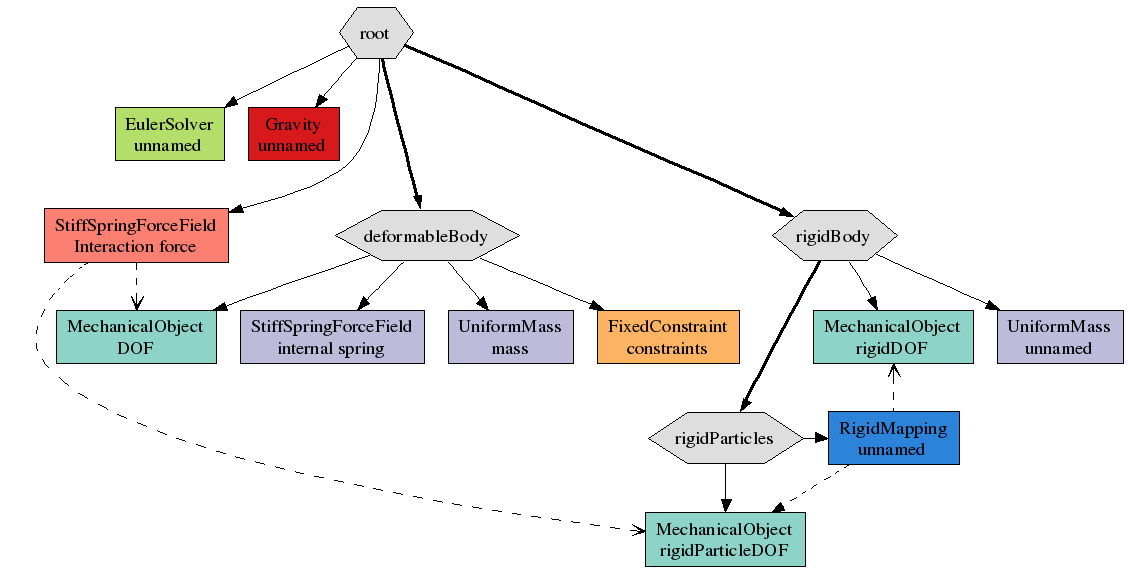
\includegraphics[width=0.9\linewidth]{mixedPendulum.png}
 \caption{A pendulum composed of a rigid body (reference frame and yellow point) attached to an elastic string (green) fixed at one end (pink point). 
 The corresponding scene graph is displayed on the left.}
 \label{fig:mixedPendulum}
\end{figure}
This scene is modeled and simulated in C++ as shown in section~\ref{cpp:hybrid}. 
The corresponding scene graph is shown in figure~\ref{fig:mixedPendulum-graph}. 
Note that the graph in the left of figure~\ref{fig:mixedPendulum} only displays a hierarchical view, while the whole graph includes additional pointers displayed as dashed arrows in figure~\ref{fig:mixedPendulum-graph}.
\begin{figure}
 \centering
 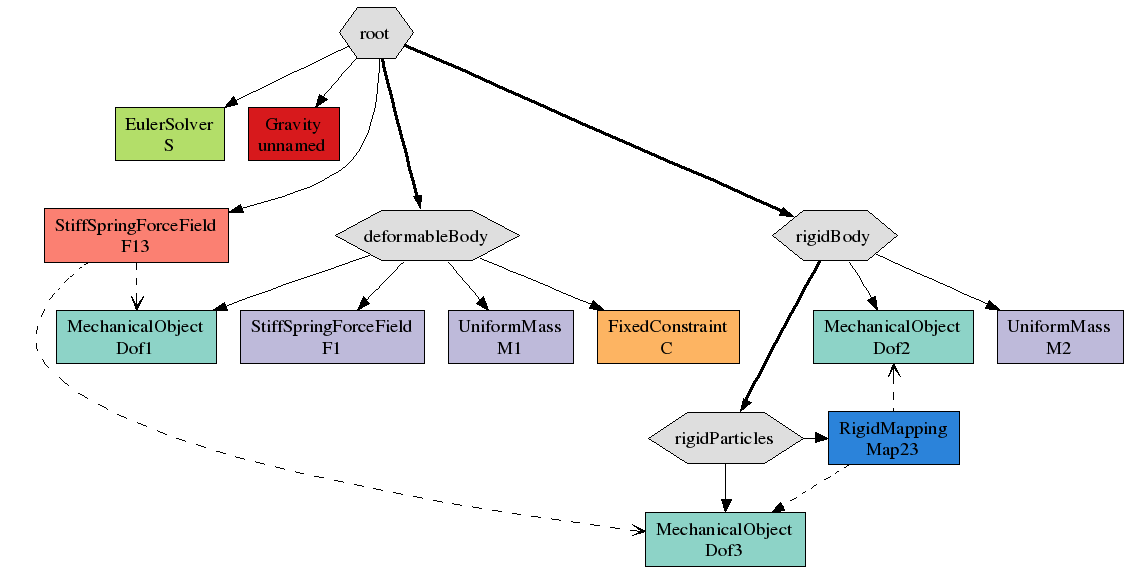
\includegraphics[width=\linewidth]{mixedPendulum-graph}
 \caption{The scene graph of the mixed pendulum. 
 The nodes are displayed as grey hexagons, while the components are displayed as rectangles with colors associated with their types or roles. 
 The bold plain arrows denote node hierarchy, while the thin plain arrows point to the components attached to the nodes, and the dotted arrows denote pointers between components.}
 \label{fig:mixedPendulum-graph}
\end{figure}

The scene is modeled as a tree structure with four nodes:
\begin{itemize}
 \item \texttt{root}
 \item \texttt{deformableBody} corresponds to the elastic string
 \item \texttt{rigidBody} corresponds to the rigid object
 \item \texttt{rigidParticles} corresponds to a set of particles (only one in this case) attached to the rigid body
\end{itemize}
Each node can have children nodes and \textit{components}. 
Each component implements a reduced set of functionalities.


One of the most important type of component is the \texttt{MechanicalObject}, which contains a list of \textit{degrees of freedom} (DOF), i.e. coordinates, velocities, and associated auxiliary vectors such as forces and accelerations.
All the coordinates in a \texttt{MechanicalObject} have the same type, e.g. 3D vectors for particles, or (translation, rotation) pairs for rigid bodies. 
\texttt{MechanicalObject}, like many other \sofa{} classes, is a generic (C++ template) class instantiated on the types of DOF it stores.
The particle DOFs are drawn as white points, whereas the rigid body DOFs are drawn as red, green, blue reference frame axes.
There can be at most one \texttt{MechanicalObject} attached to a given node. 
This guarantees that all the components attached to the same node process the same types of DOF. 
Consequently, the particles and the rigid body necessarily belong to different nodes.

In this example, the masses are stored in \texttt{UniformMass} components.
The types of their values are related to the types of their associated DOF.
\texttt{UniformMass} is derived from the abstract \texttt{Mass} class, and stores only one value, for the case where all the associated objects have the same mass. 
If necessary, it can be replaced by a \texttt{DiagonalMass} instantiated on the same DOF types, for the case where the associated objects have different masses. 
This is an important feature of \sofa: each component can be replaced by another one deriving from the same abstract class and instantiated on the same DOF types. 
This results in a high flexibility.

The \texttt{FixedConstraint} component attached a particle to a fixed point in world space, drawn in pink. 
The constraints act as filters which cancel the forces and displacements applied to their associated particle(s). 
They do not model more complex constraints such as maintaining three points aligned.

The \texttt{StiffSpringForceField} stores a list of springs, each of them modeled by a pair of indices, as well as the standard physical parameters, stiffness, damping and rest length.

The rigid body is connected to the deformable string by a spring.
Since this spring is shared by the two bodies, it is modeled in the \texttt{StiffSpringForceField} attached to a common ancestor, the graph root in this example.
Our springs can only connect particles. 
We thus need to attach a particle to the rigid body. 
Since the particle DOFs types are different from the rigid body DOF types, they have to be stored in another \texttt{MechanicalObject}, called \texttt{rigidParticleDOF} in this example, and attached to a different node.
However, \texttt{rigidParticleDOF} is not a set of independent DOF, since they are fixed in the reference frame of the rigid body. We thus attach it to a child node of the rigid body, and connect it to \texttt{rigidDOF} using a \texttt{RigidMapping}. 
This component stores the coordinates of the particle in the reference frame of the rigid body. 
Its task is to propagate the position, velocity and displacement of the rigid body down to the yellow particle, and conversely, to propagate the forces applied to the particle up to the rigid body.

Mappings are one of the major features of \sofa. 
They allow us to use different geometric models for a given body, e.g. a coarse tetrahedral mesh for viscoelastic internal forces, a set of spheres for collision detection and modeling, and a fine triangular mesh for rendering.

The gravity applied to the scene is modeled in the \texttt{Gravity} component near the root. 
It applies to all the scene, unless locally overloaded by another gravity component inside a branch of the tree.

The abstract component classes are defined in namespace \texttt{core::componentmodel}.

So far, we have discussed the physical model of the scene.
To animate it, we need to solve an \textit{Ordinary Differential Equation} (ODE) in time.
There are plenty of ODE solvers, and \sofa{} allows the design and the re-use of a wide variety of them.
Here we use a simple explicit Euler method, modeled using an \texttt{EulerSolver} component.
It triggers computations such as force accumulation, acceleration computation and linear operations on state vectors.
More sophisticated solvers are available in \sofa, and can be used by simply replacing the  \texttt{EulerSolver} component by another one, e.g \texttt{RungeKutta4} or \texttt{CGImplicit}.

Other capabilities of \sofa, such as collision detection and response, will be discussed in subsequent sections.

\section{Multi-model objects} \label{sec:multimodel}
An important feature of Sofa is the possibility of using different models of a single physical object. Figure~\ref{fig:liver} shows a scene graph representing a liver, and three different images of it.
The liver exhibits three different geometries for mechanics, rendering and collision.
\begin{figure}
 \centering
 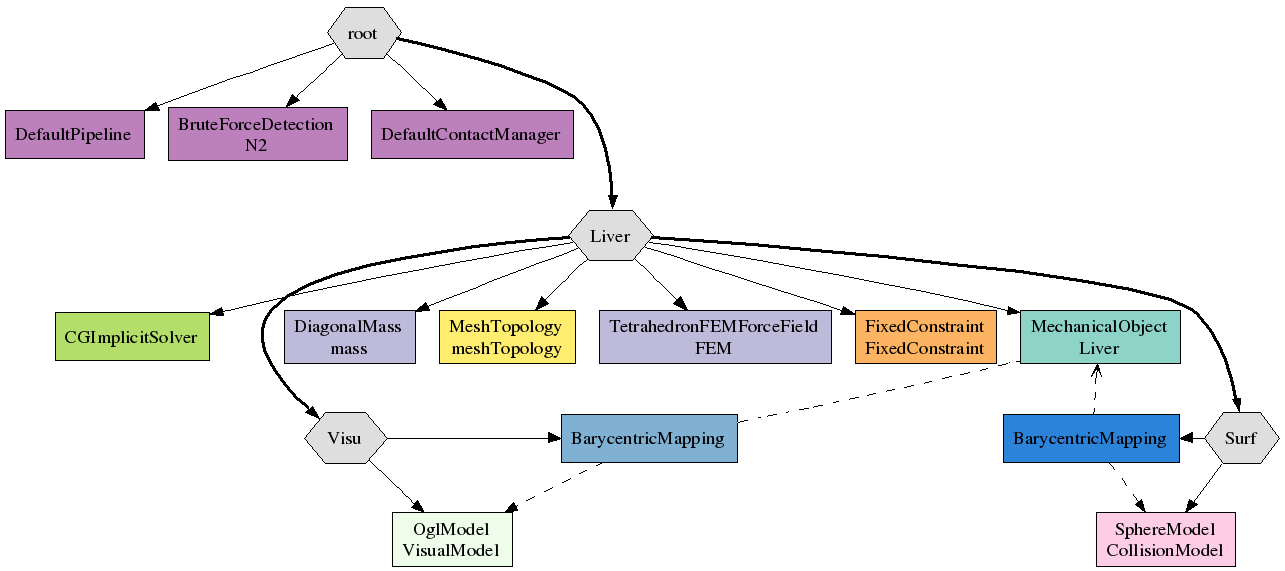
\includegraphics[width=0.95\linewidth]{liver_graph}\\
 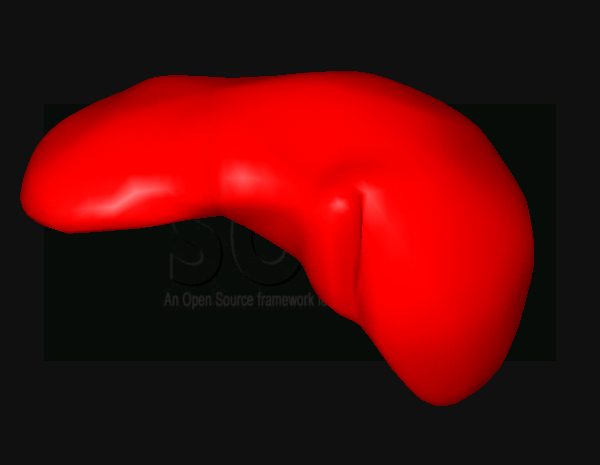
\includegraphics[width=0.3\linewidth]{liver_smooth_visu}
 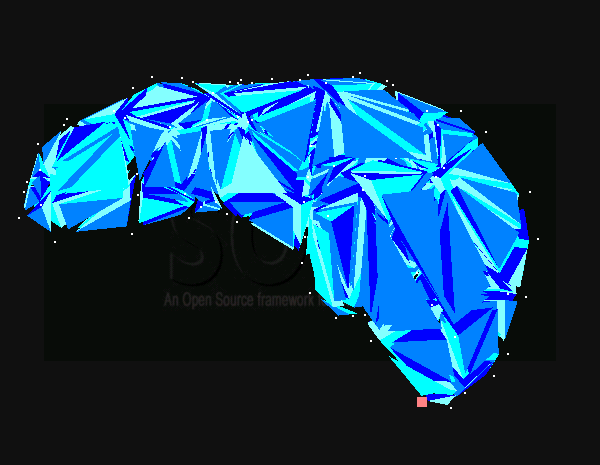
\includegraphics[width=0.3\linewidth]{liver_behavior}
 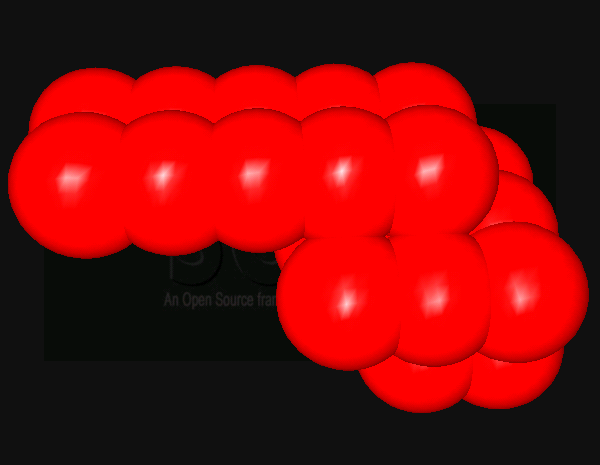
\includegraphics[width=0.3\linewidth]{liver_collision}
 \caption{A liver. Top: scene graph. Bottom: visual model, mechanical model, collision model, respectively.}
 \label{fig:liver}
\end{figure}
The corresponding xml code is given in section~\ref{xml:liver}.
\label{bla:liver}

On top of the scene, collision-related components allow a user to interact with the collision models using rays cast from the mouse pointer and hitting collision models. 
%Collision is discussed in section~\ref{sec:collision}.

The liver is modeled using three nodes, in two levels. 
The parent level contains the mechanical DOFs (particle positions and velocities) in a \texttt{MechanicalObject} component. 
These DOFs are the mechanically independent degrees of freedom of the object, in Lagrange's formalism. 
The node also contains components related to the dynamics of the particles, such as mass and internal forces. 
We call it the \textit{behavior model}.

The two other nodes are in the lower level because during the simulation, their coordinates are totally defined by the coordinates of their parent node. 
Thus, they do not belong to the set of mechanically independent DOFs. 
\emph{Mappings} are used to compute their positions and velocities based on their parent's, using the pointers represented as dashed arrows. 
Mappings are not symmetric. 
The motion of the parent DOFs is mapped to the children DOFs, whereas the motion of the children DOFs is not mapped to their parent. 
This ensures consistency.

The \texttt{VisualModel} has vertices which are used for rendering, along with other rendering data such as a list of polygons, normals, etc. 
The mapping is one-way and the mapped DOFs have no mechanical influence.

The \texttt{SphereModel} class derives from \texttt{MechanicalObject}, with an additional radius value. 
It also derives from \texttt{CollisionModel}, which allows it to be processed by the collision detection and modeling pipeline. 
When contact or mouse interaction forces are applied to the spheres, the forces are propagated bottom-up to their parent DOFs by the mapping (see section~\ref{sec:mappings}). 
This allows the contact forces to be taken into account in the dynamics equations. 
The mapping is thus two-ways and derives from \texttt{MechanicalMapping} instead of \texttt{Mapping}. 
This is why it has a different color in the image of the scene graph.
Again, the mechanical mappings are not symmetric: the forces are propagated from the children to the parents, not the other way round.

Mappings only propagate positions top-down, whereas MechanicalMappings additionally propagate velocities top-down and forces bottom-up.

Mapped models can be designed independently of their parent models, provided that the adequate (mechanical) mapping is available. 
This results in a high flexibility. 
For example, collision spheres can be replaced by collision triangles without changing anything in the behavior model or in the visual model. 
Similarly, other visual models can be used without modifying the behavior and collision models, and different behavior models can be used with the same collision and visual models, as illustrated in figure~\ref{fig:behaviormodels}.

\begin{figure}
 \centering
 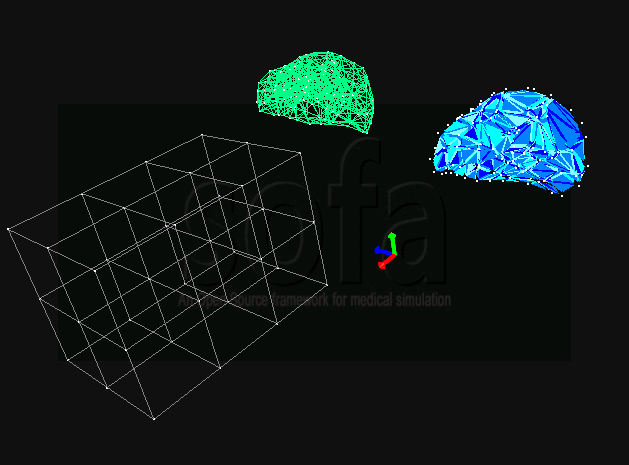
\includegraphics[width=0.4\linewidth]{demoLiverFall1.png}
 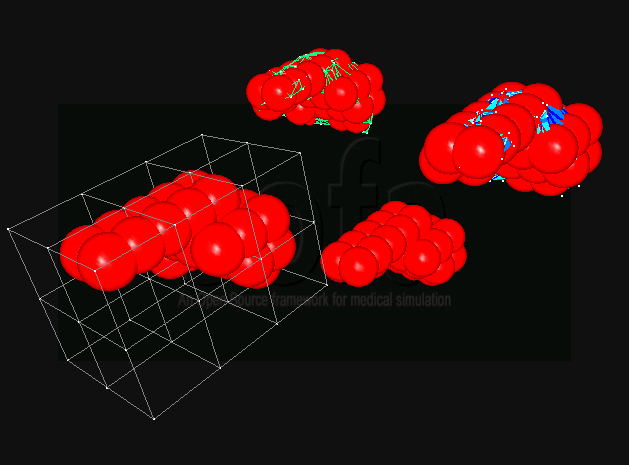
\includegraphics[width=0.4\linewidth]{demoLiverFall2.png}
 % demo.: 1179666x1179666 pixel, 0dpi, infxinf cm, bb=
 \caption{Left: four behavior models (from left to right: deformable grid, springs, rigid, tetrahedral FEM) combined with the same collision model (right).}
 \label{fig:behaviormodels}
\end{figure}


\section{Recursive data processing}
A typical simulation program, controlled by an application such as the Graphics User Interface (GUI), looks like the one given in figure~\ref{pc:animationloop}.
\begin{figure}
\begin{code_cpp}
init();
repeat {
    animate();
    draw();
}
\end{code_cpp}
\caption{Pseudocode for a standard simulation program.}
\label{pc:animationloop}
\end{figure}
In \sofa, each of the simulation methods is implemented as a recursive graph traversal, \texttt{InitVisitor}, \texttt{AnimateVisitor} and \texttt{VisualDrawVisitor}, respectively. 
Visitors are explained in the next section.

\subsection{Visitors}
The data structure is processed using objects called \emph{visitors}.
They recursively traverse the tree structure and call appropriate virtual methods to a subset of components during the \textit{Top-Down Traversal} (TDT), using virtual method \texttt{Visitor::processNodeTopDown}, then during the \textit{Bottom-Up Traversal} (BUT), using virtual method \texttt{Visitor::processNodeBottomUp}.

For example, the \texttt{VisualDrawVisitor} draws the \texttt{VisualModel} components during the TDT, and does nothing during the BUT.
The \texttt{MechanicalComputeForceVisitor} accumulates the forces in the appropriate DOF vectors during the TDT, then propagates the forces to the parent DOFs using the mechanical mappings during the BUT.

When processed by a visitor $a$, a component can fire another visitor $b$ through its associated sub-tree. 
Visitor $a$ can continue once visitor $b$ is finished.
During the TDT, each traversed component decides whether the calling visitor continues, or prunes the sub-tree associated with the component, or terminates.

The components directly access their sibling components only, except for the mappings.
A component traversed by a visitor can indirectly access the data in its associated sub-tree in read-write mode using visitors, whereas data in its parent graph is read-only and only partially accessible using method \texttt{getContext}.
Sibling nodes of the same type can be traversed by visitors in arbitrary order.

The visitors belong to namespace \texttt{sofa::simulation}.

\subsection{ODE Solvers}
When an \texttt{AnimateVisitor} traverses a node with an \texttt{OdeSolver} component,
the solver takes the control of its associated subtree and prunes the \texttt{AnimateVisitor}. 
The solver triggers visitors in its associated subtree to perform the standard mechanical computations and integrate time.

The simplest solver is the explicit Euler method, implemented in \texttt{EulerSolver}. 
The algorithm is shown as pseudocode in figure~\ref{pc:expliciteuler}.
\begin{figure}
\begin{code_cpp}
f = 0
accumulateForces(f,x,v);
a = f/M;
a = filter(a);
x += v * dt;
v += a * dt;
\end{code_cpp}
\caption{Pseudocode for explicit Euler integration.}
\label{pc:expliciteuler}
\end{figure}
Net force is computed in the first line.
In the second line, the acceleration is deduced by dividing the force by the mass.
Then the accelerations of the fixed points are canceled.
Finally, position and velocity are updated.

This algorithm can not be directly implemented in \sofa{} because there are no state vectors x,v,f,a which gather the state values of all the objects in the scene.
The solver processes an arbitrary number of objects, of possibly different types, such as particles and rigid bodies. Each physical object carries its state values and auxiliary vectors in its own \texttt{MechanicalObject} component, which is not directly accessible to the solver.

The solvers represent state vectors as \texttt{MultiVector} objects using symbolic identificators implemented in class \texttt{VecId}.
There are four staticly predefined identificators: \texttt{VecId::position()}, \texttt{VecId::velocity()}, \texttt{VecId::force()} and \texttt{VecId::dx()}.
A \texttt{Multivector} declared by a solver with a given VecId implicitly refers to all the state vectors in the different \texttt{MechanicalObject} components with the same \texttt{VecId} in the solver's subtree.

Vector operations can be remotely triggered by a solver using a visitor of a given type, which defines the operator, and given \texttt{VecId}s, which define the operands.
During the subtree traversal, the operator is applied to the given vectors of the traversed \texttt{MechanicalObject} components.

For example, let us comment the visitors performed by the \texttt{EulerSolver} shown in figure~\ref{fig:mixedPendulum}. Its implementation is in method \texttt{component::odesolver::EulerSolver::solve(double)}.
First, multivectors are declared.

Then method \texttt{core::componentmodel::behavior::OdeSolver::computeForce(VecId)} is called. 
It first fires a \texttt{MechanicalResetForceVisitor} to reset the force vectors of all the \texttt{MechanicalObject} components. 
It then fires a  \texttt{MechanicalComputeForceVisitor}. 
During the TDT, each component derived from \texttt{core::componentmodel::behavior::BaseForceField} computes and accumulates its force in its sibling \texttt{MechanicalObject}. 
In the example shown in figure~\ref{fig:mixedPendulum}, \texttt{F13} adds its contribution to \texttt{Dof1} and \texttt{Dof3}, then \texttt{F1} and \texttt{M1} add their contributions to \texttt{Dof1}, then \texttt{M2} to \texttt{Dof2}. 
Then during the BUT, the mechanical mappings sum up the forces of their child DOF to their parent DOF, \textit{i.e.}, the force in \texttt{Dof3} to \texttt{Dof2} through \texttt{M23} in the same example.
Note that branches \texttt{deformableBody} and \texttt{rigidBody} can be processed in parallel.
At the end, the force vector in \texttt{Dof1} contains the net force applied to the particles, and the force vector in \texttt{Dof2} contains the net (six-dimensional) force applied to the rigid body.

Then method \texttt{OdeSolver::accFromF(VecId,VecId)} fires a \texttt{MechanicalAccFromFVisitor}. 
Each component derived from \texttt{core::componentmodel::behavior::BaseMass} computes the accelerations corresponding to the forces in its sibling \texttt{MechanicalObject}.

Then method \texttt{OdeSolver::projectResponse} fires a \texttt{MechanicalApplyConstraintsVisitor}. 
All the \texttt{core::componentmodel::behavior::BaseConstraint} components (component \texttt{C} in the example) filter the acceleration vector to maintain some points fixed.

Once the acceleration is computed, multivector methods are used to update the positions and velocities. 
Here again, visitors are used to perform the desired operation in each traversed \texttt{MechanicalObject}.

MultiVector operations are pruned at the first level for efficiency, because the solvers deal with the mechanically independent state variables rather than the mapped variables.
Moreover, the mapped coordinates can not be assumed to vary linearly along with their parent variables.
Applying a \\ \texttt{MechanicalPropagatePositionAndVelocityVisitor} is thus necessary to update the mapped DOFs based on the mechanically independent DOFs.
This visitor is automatically performed after time integration, as one can see in the code of method \texttt{MechanicalIntegrationVisitor::fwdOdeSolver}.
It is also used by some solvers when auxiliary states are needed, as discussed in section~\ref{sec:statevectors}, in order to update the mapped DOFs.

\todo{Call tree of AnimateVisitor, restricted to sofa::core and sofa::simulation}

\todo{Discuss independent and shared solvers}

\section{State vectors} \label{sec:statevectors}
The state vectors contain the coordinates, velocites, and other DOF-related values such as force and acceleration.
They are stored in \texttt{MechanicalObject} components.
This template class can be instantiated on a variety of types to model particles, rigid bodies or other types of bodies.
The template parameter is a \texttt{DataTypes} class which describes data and data containers, such as the the type of coordinates and coordinate derivatives used.
These two types are the same in the case of particles, but they are different in the case of rigid bodies.

Each \texttt{MechanicalObject} can represent a set of physical objects of the same type, such as particles.
The coordinate state vectors are defined by the \texttt{VecCoord} type, while the derivatives (velocity, acceleration, force, small displacement) are defined by the \texttt{VecDeriv} type.
Each \texttt{MechanicalObject} stores two arrays of state vectors, one for coordinates and the other for derivatives, as illustrated in figure~\ref{fig:mechanicalobject}.
\begin{figure}
 \centering
 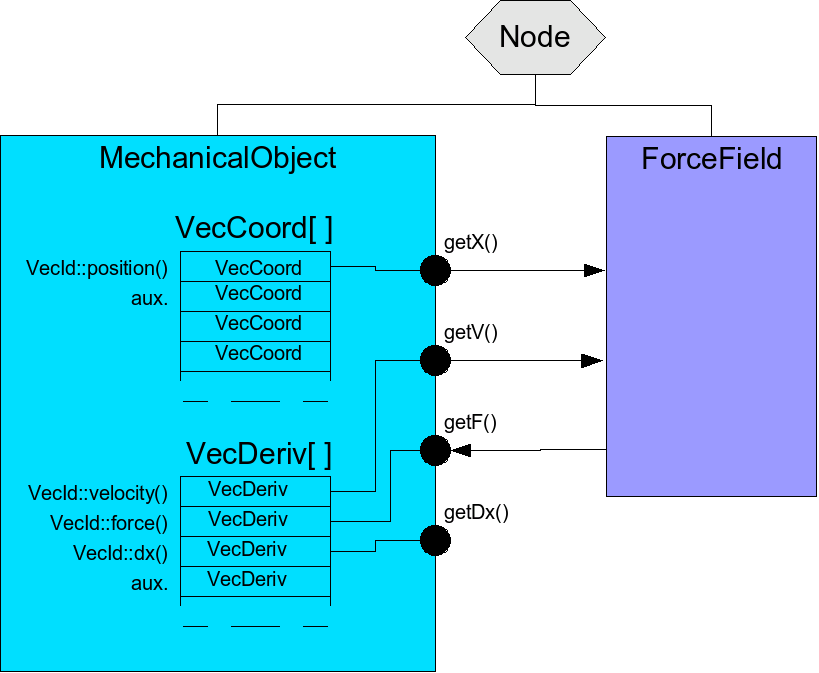
\includegraphics[width=0.45\linewidth]{MechanicalObject1}
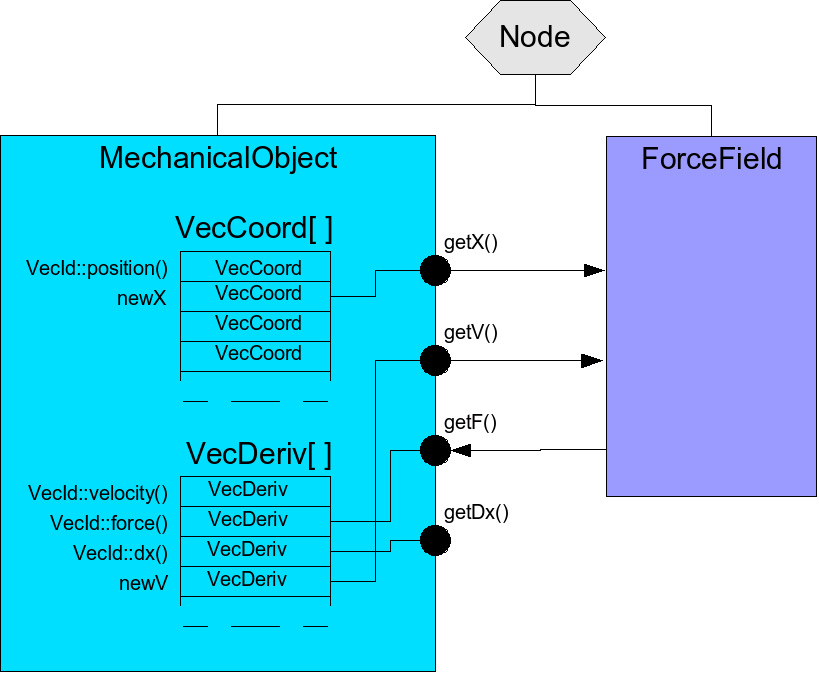
\includegraphics[width=0.45\linewidth]{MechanicalObject2}
  \caption{A \texttt{MechanicalObject} and a component addressing it. Left: using the default state vectors. Right: using auxiliary state vectors.}
 \label{fig:mechanicalobject}
\end{figure}

Auxiliary vectors are necessary for complex solvers, such as \texttt{RungeKutta2Solver}. 
This solver first performs a half-length Euler step, then evaluates the derivative of this new state (called the \emph{midpoint}), and finally uses this derivative to update the initial state over a whole time step.

To compute the forces at the midpoint while keeping the initial state for further use, we use the auxiliary vectors \texttt{newX} and \texttt{newV}.
However, components such as forces and constraints use state vectors, and we have to make sure that they use the right ones.
To ensure consistency and make the use of auxiliary states transparent, the other components get access to the state vectors using methods \texttt{MechanicalObject::getX()}, \texttt{getV()}, \texttt{getF()} and  \texttt{getDx()}.
These methods return pointers to the appropriate vectors, as illustrated in figure~\ref{fig:mechanicalobject}.

Internal  \texttt{MechanicalObject} switches are performed by methods \texttt{MechanicalObject::setX()}, \texttt{setV()}, \texttt{setF()} and  \texttt{setDx()}.
These methods are applied by the visitors which take multivectors as parameters, before they use other components. 
See, for example, method\\ \texttt{MechanicalPropagatePositionAndVelocityVisitor::fwdMechanicalState}.

Note that some constraint-based animation methods require large state vectors and matrices encompassing all the mechanical objects of the scene.
Such methods are currently under development in \sofa, and they are not yet documented.
They use visitors to count the total number of scalar DOFs and to gather them in large state vectors, as well as to build mechanical matrices  such as mass, stiffness, damping and compliance etc.

\subsection{Mechanical groups}
During the simulation, each solver prunes the \texttt{AnimateVisitor} which traverses it and manages its associated subtree by itself using other visitors.
The objects animated by a given solver are called a \emph{mechanical group}.
Each mechanical group corresponds to a subtree in the scene graph.
In the example discussed in section~\ref{sec:commentedExample}, there is one mechanical group because a single solver located near the root manages the whole scene.
However, using separate solvers for different objects can sometimes increase efficiency.
In the example shown in figure~\ref{fig:twoSolvers}, the same deformable body is animated using a \texttt{RungeKutta2Solver} while the rigid body is animated using an \texttt{EulerSolver}.
\begin{figure}
 \centering
 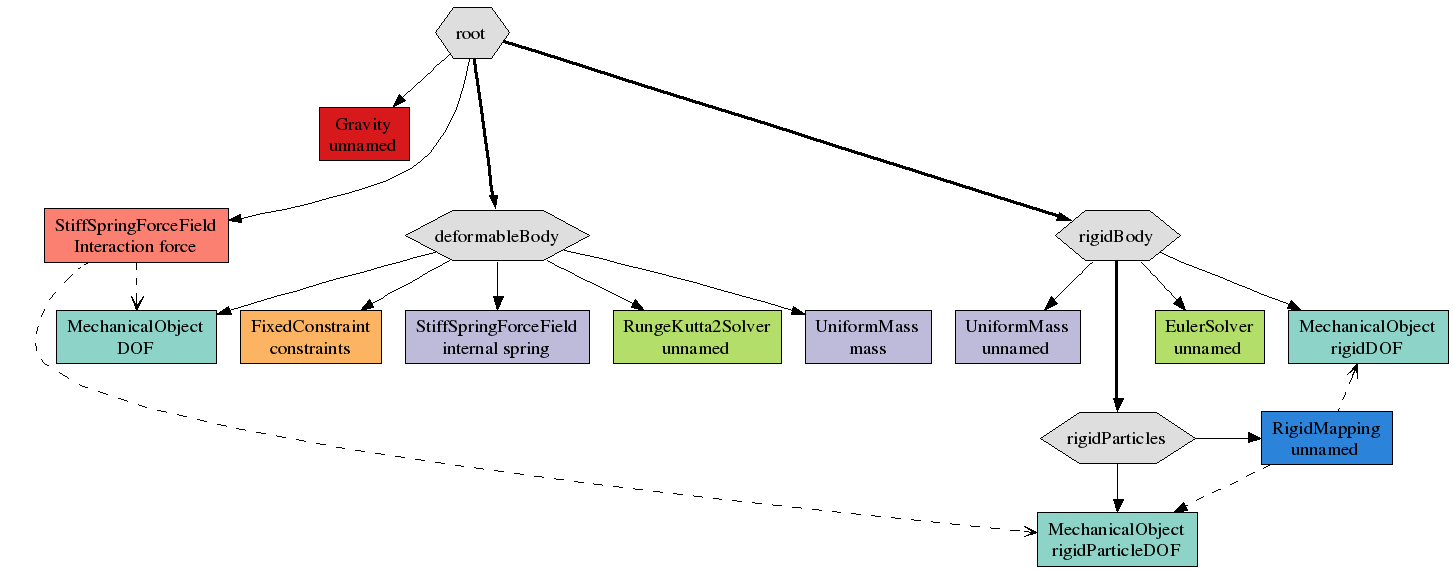
\includegraphics[width=0.95\linewidth]{twoSolvers}
  \caption{A scene graph with objects animated using different ODE solvers.}
 \label{fig:twoSolvers}
\end{figure}


A mechanical group can include interaction forces between elements of the group, and such interaction forces are handled by the solver as expected.
Interaction forces can also occur between objects which do not belong to the same group.
In this case, the interaction force is located at a higher hierarchical level than the objects it applies to, as shown in figure~\ref{fig:twoSolvers}.
It can not be traversed by visitors fired by the solvers.
Its evaluation is performed by the \texttt{AnimateVisitor}, and accumulated as external forces in the associated \texttt{MechanicalObject} components.
Consequently, it acts as a constant force during each whole animation step.
In a \texttt{RungeKutta2Solver}, during the force computation at midpoint, its value is the same as at the starting point.
In a \texttt{CGImplicitSolver}, its stiffness is not taken into account, which may introduce instabilities if its actual stiffness is high.

The default collision manager of Sofa circumvents this problem by dynamically gathering the objects in contact in a common mechanical group.

% \section{Mostly used components and methods}
% \subsection{ForceFields}
% \subsection{Constraints}
% \subsection{Masses}
% \subsection{Mappings}
% \subsection{ContextObjects}
%
% \section{Collision detection} \label{sec:collision}
%
%
% \section{Limitations}

% \pagebreak
% \appendix
\section{Code of the examples}
\subsection{The hybrid pendulum}\label{cpp:hybrid}
This is the code of the example commented in section~\ref{sec:commentedExample} :
\includecode{C++}{../../applications/tutorials/mixedPendulum/Main.cpp}

\subsection{A liver}\label{xml:liver}
The XML code of the liver discussed in section~\ref{sec:multimodel} page~\pageref{bla:liver} is in \texttt{../examples/Demos/liver.scn}

% \chapter{Animation in \sofa}\label{chapter:as}
This section shows how the material presented in chapter \ref{chapter:pba} is implemented in \sofa. A class diagram of the mechanical core is presented in appendix \ref{sec:umlmeca}.
\section{Particles}
\subsection{Simple example}
Here we simulate two particles subject to gravity. An introduction to particle dynamics is given in section \ref{sec:particles}. 
Figure \ref{fig:singleParticleCollaboration} shows the collaboration diagram and the code used to model a set of particles subject to gravity. The code is available in project {\tt doc/src\_examples/example1}.


\begin{figure}[htp]
\begin{center} \begin{tabular}{cc}
\begin{minipage}[b]{6cm}
	\includegraphics*[width=6cm]{fig/singleParticleCollaboration.eps}  
	%\input{fig/singleParticleCollaboration.tex} 
\end{minipage}
 &
\begin{minipage}[b]{9cm} 
\begin{code_cpp}
#include "Sofa/Components/Scene.h"
#include "Sofa/Components/MassObject.h"
#include "Sofa/Components/EulerSolver.h"
#include "Sofa/GUI/FLTK/Main.h"

using namespace Sofa::Components;
using namespace Sofa::Core;
using namespace Sofa::GUI::FLTK;
typedef Sofa::Components::Common::Vec3Types MyTypes;
typedef MyTypes::Deriv Vec3;
        
int main(int argc, char** argv) 
{
    Scene* scene = new Scene;
    scene->setDt(0.04);
    
    MechanicalGroup* group = new MechanicalGroup;
    scene->addBehaviorModel(group);
    group->setSolver( new EulerSolver );
    
    MassObject<MyTypes>* particles = new MassObject<MyTypes>;
    group->addObject(particles);
    scene->addVisualModel(particles);                 
    particles->setGravity( Vec3( 0,-1,0 ) );
    particles->addMass( Vec3(2,0,0), Vec3(0,0,0), 1 ); 
    particles->addMass( Vec3(3,0,0), Vec3(0,0,0), 1 );


    scene->init();
    MainLoop(argv[0]);
    return 0;
}
\end{code_cpp}
\end{minipage}
\end{tabular}
\end{center}
\label{fig:singleParticleCollaboration} 
\caption{Collaboration diagram and code for the animation of free particles.}
\end{figure}


%
% \chapter{Extending \sofa}\label{chapter:es}

This chapter presents how different types of classes can be added to \sofa{} to implement new behaviors.

\section{Adding a new DynamicObject}

A DynamicObject is responsible for implementing the behavior of a given type of body. It contains the degrees of freedoms (\textit{DOFs}) of the body (within the MechanicalObject class), as well as its mass (i.e. how the body moves given an applied force).

To add a new DynamicObject in \sofa, the following steps are required:

\begin{enumerate}
\item Specify the type of its DOFs in a \textcode{DataTypes} class.
\item Create the \textcode{DynamicObject} derived class implementing the behaviors of the body, or instantiate an existing class with you \textit{DataTypes} class if already available.
\item Create a method to create an instance of the body given an XML node.
\item Register the new DynamicObject in the \textcode{Sofa::Components::XML::DynamicNode::Factory} factory.
\item Create a XML scene file containing a DynamicModel with the \textit{type} of our class.
\item Have fun!
\end{enumerate}

If the new class will only be created procedurally, then only the first two steps are required.

We will now detail these steps using the example of an object containing a set of one-dimensional particles.

The code corresponding to this example is available in the following files:
\begin{description}
\item[Sofa/doc/src\_examples/example3/MassObject1d.h]~\\
 Declaration of MassObject1d.
\item[Sofa/doc/src\_examples/example3/MassObject1d.cpp]~\\
 Creation from XML and registration in the Factory
\item[Sofa/doc/src\_examples/example3/Main.cpp]~\\
 Main program
\item[Sofa/doc/src\_examples/example3/test1.scn]~\\
 Test scene file
\end{description}

\subsection{Specification of the Degrees of Freedom}\label{sec:DOF}

The data types used by the body are specified in a class containing the following definitions:

\begin{description}
\item[Coord]~\\
 Type of DOFs.
\item[Deriv]~\\
 Type of derivatives (velocity, forces, displacements).
\item[VecCoord]~\\
 Container of DOFs.
\item[VecDeriv]~\\
 Container of derivatives.
\item[void set(Coord\& c, double x, double y, double z)]~\\
 Utility method to set the value of a point.
\item[void add(Coord\& c, double x, double y, double z)]~\\
 Utility method to add a value to a point (for applyTranslation).

\end{description}

In our example, we can use double as the type of DOFs and std::vector as containers:

\begin{code_cpp}
class Vec1dTypes
{
public:
  typedef double Coord;
  typedef double Deriv;
  typedef std::vector<Coord> VecCoord;
  typedef std::vector<Deriv> VecDeriv;
  
  /// Here we only use the first coordinate
  static void set(Coord& c, double x, double /*y*/, double /*z*/)
  {
    c = x;
  }
  
  static void add(Coord& c, double x, double /*y*/, double /*z*/)
  {
    c += x;
  }
};
\end{code_cpp}

\subsection{Body Behaviors Implementation}

In \sofa{} a DynamicObject does not implement the time integration algorithm, which is handled by an separate Solver. Instead, it implements basic operations, such as compute forces, combine several vectors, etc. Of these operations, most are only dependant on the types of DOFs, or are computed through external classes (ForceFields for instance). Only 3 operations related to the mass remain to be implemented by DynamicObject subclasses:

\begin{description}
\item[computeForce] must be modified to add gravity ( $\ve f = \ve f + \ma M \ve g$ ).
\item[accFromF] must be implemented to convert forces to accelerations ( $\ve a = \ma M^{-1} \ve f$ ).
\item[addMDx] must be implemented to multiply a given displacement by the mass ( $ \ve r = \ve r + \ma M \ve dx$ ).
\end{description}

In our example, a class \textcode{MassObject} already exists to handle object represented as a set of particles. So we just need to instantiate it to the type of DOFs we want to use:

\begin{code_cpp}
typedef MassObject<Vec1dTypes> MassObject1d;
\end{code_cpp}

As a reference, here is how MassObject implements the 3 operations mentioned earlier:

\begin{code_cpp}
template <class DataTypes>
void MassObject<DataTypes>::addMDx(VecDeriv* res, VecDeriv* dx)
{
  for( unsigned i=0; i<dx->size(); ++i )
    (*res)[i] += (*dx)[i] * masses[i].mass;
}


template <class DataTypes>
void MassObject<DataTypes>::accFromF(VecDeriv* a, VecDeriv* f)
{
  a->resize(f->size());
  for( unsigned i=0; i<f->size(); ++i )
    (*a)[i] = (*f)[i] / masses[i].mass;
}


template <class DataTypes>
void MassObject<DataTypes>::computeForce(VecDeriv* result)
{
  Inherit::computeForce(result);
  // Add Gravity
  for (unsigned int i=0;i<result->size();i++)
  {
    (*result)[i]+=gravity*masses[i].mass;
  }
}
\end{code_cpp}

\subsection{Instantiation from XML}

\sofa{} implements a mechanism to load a scene from a XML file using a two step process:

\begin{enumerate}
\item The XML file is parsed and converted to a tree of Node class.
\item Each node use a Factory to instantiate the described object.
\end{enumerate}

A DynamicObject is described by a \textcode{Sofa::Components::XML::DynamicNode}. It contains the type of the class to instantiate, as well as a set of string attributes. To build our DynamicObject from this description we need a function to construct and configure a new instance given the pointer to the XML::DynamicNode. This can either be a constructor in our class, or an external function with the following prototype:
\begin{code_cpp}
namespace Sofa { namespace Components { namespace Common {
void create(MyDynamicObject*& obj, XML::Node<Sofa::Abstract::DynamicModel>* arg);
} } }
\end{code_cpp}
where \textcode{MyDynamicObject} is the name of our new class.

\textbf{Note:} the inclusion in the \textcode{Sofa::Components::Common} namespace is necessary for the Factory class to find our function. If anyone find a better design removing this requirement please tell me!

Typically, the object will either be constructed from attributes given in the XML node, or using an external description file.

Our 1D particles example is simple enough not to require an external file. We can implement a creation function as follow:

\begin{code_cpp}
/// Read a vector of scalars from a string.
void readVec1(std::vector<double>& vec, const char* str)
{
  vec.clear();
  if (str==NULL) return;
  const char* str2 = NULL;
  for(;;)
  {
    double v = strtod(str,(char**)&str2);
    std::cout << v << std::endl;
    if (str2==str) break;
    str = str2;
    vec.push_back(v);
  }
}

namespace Sofa { namespace Components { namespace Common {
/// Construct a MassObject1d object from a XML node.
void create(MassObject1d*& obj, XML::Node<Sofa::Abstract::DynamicModel>* arg)
{
        obj = new MassObject1d();
  obj->clear();
  std::vector<double> mass;
  std::vector<double> pos;
  std::vector<double> vel;
  std::vector<double> fixed;
  readVec1(mass,arg->getAttribute("mass"));
  readVec1(pos,arg->getAttribute("position"));
  readVec1(vel,arg->getAttribute("velocity"));
  readVec1(fixed,arg->getAttribute("fixed"));
  if (arg->getAttribute("gravity"))
  {
    obj->setGravity(atof(arg->getAttribute("gravity")));
  }
  unsigned int maxsize = mass.size();
  if (pos.size()>maxsize) maxsize = pos.size();
  if (vel.size()>maxsize) maxsize = vel.size();
  double defaultmass = (mass.empty()?1.0:*mass.rbegin());
  while (mass.size()<maxsize)
    mass.push_back(defaultmass);
  double defaultpos = 0;
  if (!pos.empty()) defaultpos = *pos.rbegin();
  while (pos.size()<maxsize)
    pos.push_back(defaultpos);
  double defaultvel = 0;
  if (!vel.empty()) defaultvel = *vel.rbegin();
  while (vel.size()<maxsize)
    vel.push_back(defaultvel);
  for (unsigned int i=0;i<maxsize;i++)
  {
    obj->addMass(pos[i], vel[i], mass[i], 0.0,
      (std::find(fixed.begin(), fixed.end(), (double)i)!=fixed.end()));
  }
} } } }
\end{code_cpp}

Note that this function is quite long, as it construct vectors of values (masses, positions, velocities) from strings. For simpler cases, where only a filename is required for instance, generic creation functions are provided:
\begin{code_cpp}
namespace Sofa { namespace Components { namespace Common {
/// Construct a MassObject1d object from a XML node using an external file.
void create(MassObject1d*& obj, XML::Node<Sofa::Abstract::DynamicModel>* arg)
{
  XML::createFromFilename(obj, arg);
} } } }
\end{code_cpp}
However it is then necessary to implement the external file loading method.

\subsection{Factory Registration}

Once all functionalities are implemented, it is necessary to register the new class in the \textcode{Sofa::Components::XML::DynamicNode::Factory} factory in order for \sofa{} to know about it. This requires adding the following "magic" line:

\begin{code_cpp}
Creator< XML::DynamicNode::Factory, MassObject<Vec1dTypes> >
  MassObject1dClass("MassObject1d");
\end{code_cpp}

This command will register our class to the Factory during the initialization of the program. For this to work we must still ensure our code is linked in the final binary. To do this we must add the following line in the .cpp file containing the Creator command:
\begin{code_cpp}
\end{code_cpp}
and then add a corresponding line in a .cpp file used during the execution of the program (such as the file containing the main() function, or in Sofa/Components/init.cpp if the new class is integrated in \sofa{}):
\begin{code_cpp}
SOFA_INIT_CLASS(MassObject1d)
\end{code_cpp}
This last step is required to work around portability issues, and might be removed if a better solution is found.

When the given type name is used in an XML file, the Factory will now be able to construct our custom DynamicObject.

\subsection{Testing}

Our new class can now be loaded by writing a small XML file:

\begin{code_xml}
<Scene dt="0.005" showBehaviorModels="1" showCollisionModels="1" showMappings="1" showForceFields="1">
	<Group>
		<Solver type="RungeKutta4"/>
		<DynamicModel type="MassObject1d" name="M1" position="0 1 2 3 4 5" fixed="5" gravity="-9.8"/>
	</Group>
</Scene>
\end{code_xml}

To run it, go to \textcode{Sofa/doc/src\_examples/example3} and execute
\begin{code_bash}
./run test1.scn
\end{code_bash}

\begin{figure}
\centering
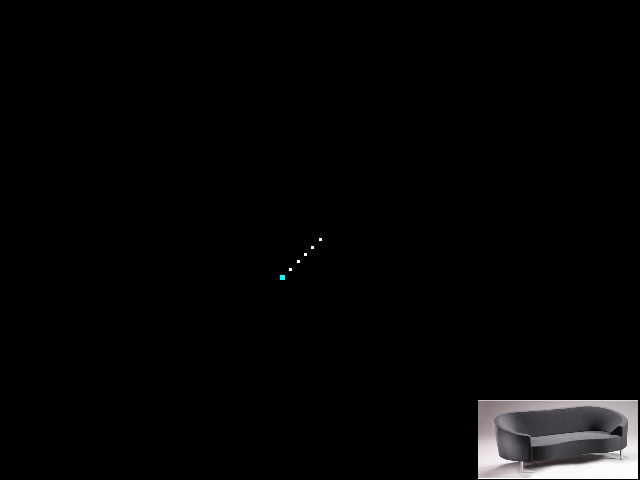
\includegraphics[width=0.5\linewidth]{fig/mass1d}
\caption{Test scene with 6 1D particles.}
\end{figure}

\section{Adding a new Mapping}

Many existing objects in \sofa{} expect to work with 3D particles. To be able to use them with our 1D particles, we can create a MechanicalMapping which will convert information between the two representations.

Adding a new Mapping in \sofa{} requires the following steps:

\begin{enumerate}
\item Create the \textit{Mapping} or \textit{MechanicalMapping} derived class computing the mapping from the input model to the output, and accumulating forces back for MechanicalMappings.
\item Create a method to create an instance of the mapping given an XML node.
\item Register the new mapping in the Sofa::Components::XML::MappingNode::Factory factory.
\item Create a XML scene file containing a Mapping with the \textit{type} of our class.
\item Have more fun!
\end{enumerate}

We will now detail these steps using the 1D to 3D mechanical mapping example.
The code for this mapping is available in the \textcode{Sofa/doc/src\_examples/example3/LinearMapping.cpp} file.

\subsection{Mapping Implementation}

A MechanicalMapping is used in the scene to link two MechanicalObjects, an input model and an output model. Positions, velocities and displacements are propagated from the input model to the output, and forces are accumulated in the other direction. This can be implemented by overloading 3 methods:

\begin{description}
\item[apply] compute output positions from input ones
\item[applyJ] compute output derivatives (velocity of displacement) from input ones
\item[applyJT] accumulate back output forces (or df) into input ones
\end{description}

If the mapping is linear these operations can be expressed in terms of the mapping matrix $\ma J$: apply and applyJ are equivalent to ${\mathbf {out}} = \ma J {\mathbf {in}}$, and applyJT is equivalent to $ {\mathbf {in}} += \ma {J^{t}} {\mathbf {out}} $.

A scene in \sofa{} can contain mechanical models with different types of degrees of freedoms (see section~\ref{sec:DOF}). The mapping can either be generic relatively to the types used in the input and output models, or requires them to use specific types. The first solution requires the mapping implementation to be declared as a template of the type of DOFs, while the second solution requires implementing a "standard" class.

For our example, we will create a non-templated mapping for simplicity, although a templated version would be very similar.

\begin{code_cpp}
class LineMapping : public Sofa::Core::MechanicalMapping< Sofa::Core::MechanicalObject<Vec1dTypes>, Sofa::Core::MechanicalObject<Vec3dTypes> >
{
public:
  // Simplified notation for all involved classes
  typedef Sofa::Core::MechanicalMapping< Sofa::Core::MechanicalObject<Vec1dTypes>, Sofa::Core::MechanicalObject<Vec3dTypes> > BaseMapping;
  typedef BaseMapping::In In;
  typedef BaseMapping::Out Out;
  typedef Out::VecCoord VecCoord;
  typedef Out::VecDeriv VecDeriv;
  typedef Out::Coord Coord;
  typedef Out::Deriv Deriv;

  Coord p0; ///< Origin of the 3D line
  Deriv dx; ///< Direction of the 3D line
  
  LineMapping(In* from, Out* to, const std::string& /*name*/)
  : BaseMapping(from, to), p0(0,0,0), dx(1,0,0)
  {
  }
  
  void apply( Out::VecCoord& out, const In::VecCoord& in )
  {
    out.resize(in.size());
    for(unsigned int i=0;i<out.size();i++)
      out[i] = p0+dx*in[i];
  }
  
  void applyJ( Out::VecDeriv& out, const In::VecDeriv& in )
  {
    out.resize(in.size());
    for(unsigned int i=0;i<out.size();i++)
      out[i] = dx*in[i];
  }
  
  void applyJT( In::VecDeriv& out, const Out::VecDeriv& in )
  {
    for(unsigned int i=0;i<out.size();i++)
      out[i] += dx*in[i];
  }
};
\end{code_cpp}

\subsection{Instantiation from XML and Registration in Factory}

This process is identical to the corresponding steps in the DynamicObject case, except that the XML Node to use is XML::MappingNode instead of XML::DynamicNode.

In our example, the additional code required for this step is:
\begin{code_cpp}

namespace Sofa { namespace Components { namespace Common {

void create(LineMapping*& obj, XML::Node<Sofa::Core::BasicMapping>* arg)
{
  XML::createWith2Objects< LineMapping, LineMapping::In, LineMapping::Out>(obj, arg);
  if (obj!=NULL)
  {
    obj->p0[0] = atof(arg->getAttribute("x0","0"));
    obj->p0[1] = atof(arg->getAttribute("y0","0"));
    obj->p0[2] = atof(arg->getAttribute("z0","0"));
    obj->dx[0] = atof(arg->getAttribute("dx","1"));
    obj->dx[1] = atof(arg->getAttribute("dy","0"));
    obj->dx[2] = atof(arg->getAttribute("dz","0"));
  }
} } } }

Creator< XML::MappingNode::Factory, LineMapping > LineMappingClass("LineMapping", true);
\end{code_cpp}

Note the true argument in the Creator command. It means that other classes with the same type name are authorized in the Factory, implementing the same mapping for other datatypes for instance.

\subsection{Testing}

Our new class can now be used to add a 3D spring force field to our 1D masses by writing a small XML file:

\begin{code_xml}
<Scene dt="0.005" showBehaviorModels="1" showCollisionModels="1" showMappings="1" showForceFields="1">
	<Group>
		<Solver type="RungeKutta4"/>
		<DynamicModel type="MassObject1d" name="M1" position="0 1 2 3 4 5" fixed="5" gravity="-9.8">
		<MechanicalModel type="Vec3d" name="Points">
		<ForceField type="StiffSpringForceField" filename="test2.xs3"/>
		</MechanicalModel>
		<Mapping type="LineMapping" input="@." output="@Points" />
		</DynamicModel>
	</Group>
</Scene>
\end{code_xml}

To run it, go to \textcode{Sofa/doc/src\_examples/example3} and execute
\begin{code_bash}
./run test2.scn
\end{code_bash}

The same mapping can also be used to attach a collision model:

\begin{code_xml}
<Scene dt="0.005" showBehaviorModels="1" showCollisionModels="1" showMappings="1" showForceFields="1">
	<CollisionPipeline>
		<CollisionDetection name="N2" type="BruteForce" />
		<Contact name="Response" response="penality" />
		<CollisionGroup name="Group" />
	</CollisionPipeline>
	<Group>
		<Solver type="RungeKutta4"/>
		<DynamicModel type="MassObject1d" name="M1" position="0 1 2 3 4 5" fixed="5" gravity="-9.8">
		<MechanicalModel type="Vec3d" name="Points">
		<ForceField type="StiffSpringForceField" filename="test2.xs3"/>
		</MechanicalModel>
		<Mapping type="LineMapping" input="@." output="@Points" />
		<CollisionModel type="Sphere" name="Spheres" filename="test3.sph"/>
		<Mapping type="LineMapping" input="@." output="@Spheres" />
		</DynamicModel>
	</Group>
</Scene>
\end{code_xml}

To run it, go to \textcode{Sofa/doc/src\_examples/example3} and execute
\begin{code_bash}
./run test3.scn
\end{code_bash}

\begin{figure}
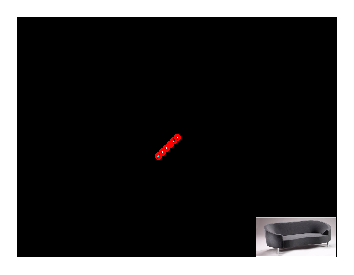
\includegraphics[width=0.5\linewidth]{fig/mass1d-collision1}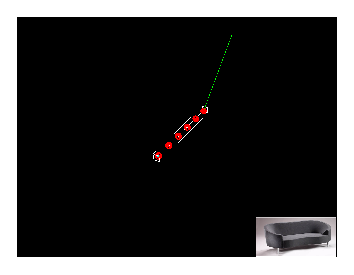
\includegraphics[width=0.5\linewidth]{fig/mass1d-collision2}
\caption{Collisions with 1D particles used to interact with the mouse.}\label{fig:mass1d-collision}
\end{figure}

\begin{figure}
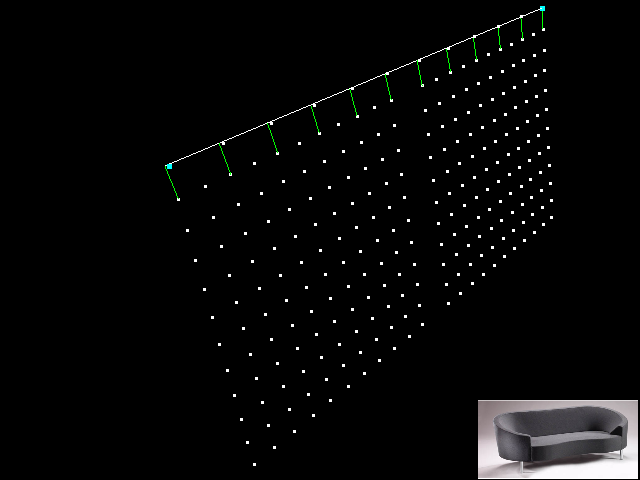
\includegraphics[width=0.5\linewidth]{fig/mass1d-curtain1}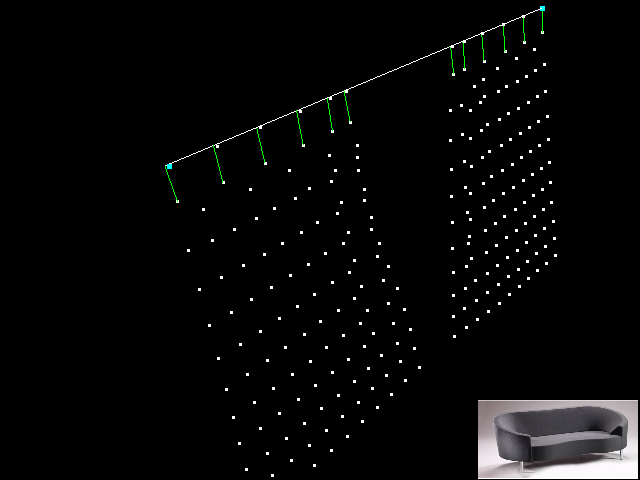
\includegraphics[width=0.5\linewidth]{fig/mass1d-curtain2}\\
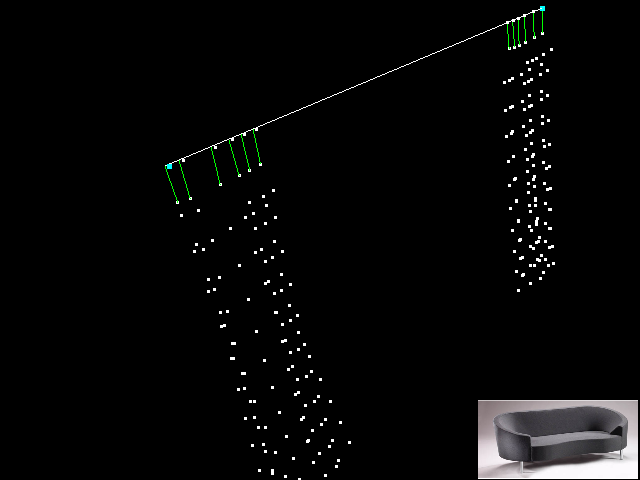
\includegraphics[width=0.5\linewidth]{fig/mass1d-curtain3}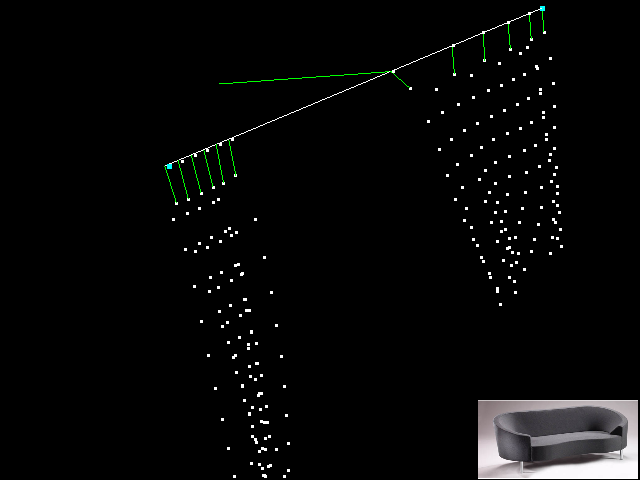
\includegraphics[width=0.5\linewidth]{fig/mass1d-curtain4}%
\caption{1D and 3D particles linked by springs to simulate curtains.}\label{fig:mass1d-curtain}
\end{figure}

You can now pick the particles with the mouse by pressing the shift key and left mouse button, as seen in figure~\ref{fig:mass1d-collision}.

The main advantage of our mapping is that we can combine 1D and 3D particles in the same simulation with forces such as springs applied between them. This is demonstrated in the \texttt{test4.scn} scene, as seen in figure~\ref{fig:mass1d-curtain}.

\section{Non-Linear Mapping}

Mappings are not limited to linear computations. Non-linear mappings can be computed exactly in the apply method, and a local linear approximation can be used for the applyJ and applyJT methods.

For instance, our 1D particles can be mapped to a circle instead of a line. The code for this mapping is available in the
\textcode{Sofa/doc/src\_examples/example3/CircleMapping.cpp} file. It uses the following computations :

\begin{description}
\item[apply] $ \ve x_{out} = \ve{p_0} + \ve{r_x} cos( \ve x_{in} ) + \ve{r_y} sin( \ve x_{in} ) $
\item[applyJ] $ \ve v_{out} = \frac{\delta \ve x_{out}}{\delta \ve x_{in}} \ve v_{in} = ( - \ve{r_x} sin ( \ve x_{in} ) + \ve{r_y} cos ( \ve x_{in} ) ) \ve v_{in} $
\item[applyJT] $ \ve f_{in} = \frac{\delta \ve x_{out}}{\delta \ve x_{in}} \ve f_{out} $ and $ \frac{\delta \ve f_{in}}{\delta \ve x_{in}} = \frac{\delta \ve x_{out}}{\delta \ve x_{in}^2} \ve f_{out} + \frac{\delta \ve x_{out}}{\delta \ve x_{in}} \frac{\delta \ve f_{out}}{\delta \ve x_{out}} $
\end{description}

Note that if we use a local linear approximation, $ \frac{\delta \ve x_{out}}{\delta \ve x_{in}^2} = 0 $ so applyJT is the same for f and df.

\begin{code_cpp}
class CircleMapping : public Sofa::Core::MechanicalMapping< Sofa::Core::MechanicalObject<Vec1dTypes>, Sofa::Core::MechanicalObject<Vec3dTypes> >
{
public:
  // Simplified notation for all involved classes
  typedef Sofa::Core::MechanicalMapping< Sofa::Core::MechanicalObject<Vec1dTypes>, Sofa::Core::MechanicalObject<Vec3dTypes> > BaseMapping;
  typedef BaseMapping::In In;
  typedef BaseMapping::Out Out;
  typedef Out::VecCoord VecCoord;
  typedef Out::VecDeriv VecDeriv;
  typedef Out::Coord Coord;
  typedef Out::Deriv Deriv;

  Coord p0; ///< Origin of the circle
  Deriv rx, ry; ///< Radius of the circle
  
  std::vector<Deriv> dx;
  
  CircleMapping(In* from, Out* to, const std::string& /*name*/)
  : BaseMapping(from, to), p0(0,0,0), rx(1,0,0), ry(0,0,1)
  {
  }
  
  void apply( Out::VecCoord& out, const In::VecCoord& in )
  {
    out.resize(in.size());
    dx.resize(in.size());
    for(unsigned int i=0;i<out.size();i++)
    {
	  double c = cos(in[i]);
	  double s = sin(in[i]);
      out[i] = p0+rx*c+ry*s;
	  dx[i] = rx*(-s)+ry*c;
    }
  }
  
  void applyJ( Out::VecDeriv& out, const In::VecDeriv& in )
  {
    out.resize(in.size());
    for(unsigned int i=0;i<out.size();i++)
      out[i] = dx[i]*in[i];
  }
  
  void applyJT( In::VecDeriv& out, const Out::VecDeriv& in )
  {
    for(unsigned int i=0;i<out.size();i++)
      out[i] += dx[i]*in[i];
  }
};
\end{code_cpp}

To run it, go to \textcode{Sofa/doc/src\_examples/example3} and execute
\begin{code_bash}
./run test5.scn
\end{code_bash}

The result is visible in figure~\ref{fig:mass1d-circle}.

\begin{figure}
\centering
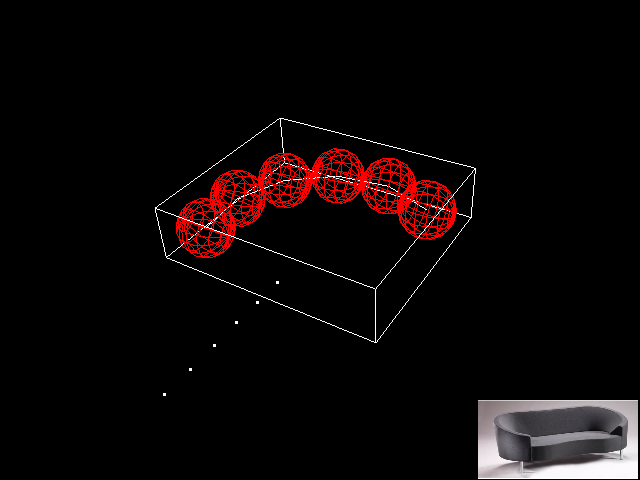
\includegraphics[width=0.5\linewidth]{fig/mass1d-circle1}
\caption{1D particles mapped to a circle.}\label{fig:mass1d-circle}
\end{figure}

\section{Adding a new ForceField}

A ForceField is used to apply forces to mechanical objects in the scene. Its basic role is to compute a force vector $\ve f$ associated with a set of DOFs, given their position $\ve x$ and velocity $\ve v$. To support implicit integration schemes, it must also compute the force derivative $\ve{df}$ given a displacement $\ve {dx}$.

Adding a new ForceField in \sofa{} requires the following steps:

\begin{enumerate}
\item Create the ForceField derived class.
\item Create a method to create an instance of the force field given an XML node.
\item Register the new force field in the \textcode{Sofa::Components::XML::ForceFieldNode::Factory} factory.
\item Create a XML scene file containing a ForceField with the \textit{type} of our class.
\item Have even more fun!
\end{enumerate}

We will now detail these steps implementing \textit{Lennard-Jones} fluid forces. It is a simple force field adding a force between any pair of particles based on a potential related to their distance $d$:\\
$potential = \dfrac{a}{d^\alpha} - \dfrac{b}{d^\beta}$\\
$f = - grad(potential) = ( a \alpha d^{-\alpha-1} - b \beta d^{-\beta-1} ) \ve u$\\
where $\ve u$ is the unit vector between the two particles. This force field has the property to force particles to stay within a certain distance of each other, and is negligible for particles far away from each other, allowing to use a cutoff distance.

Computing the Lennard-Jones forces requires $5$ parameters: $a$, $b$, $\alpha$, $\beta$, and the cutoff distance $d_{max}$. As they are not all meaningful, we will instead allow the user to specify the prefered distance $d_0$ where $f = 0$, as well as the potential value $p_0$ at this point, which controls the force magnitude. The cutoff distance $d_{max}$ will be initialized as $2 d_0$ by default, and we will use $\alpha=6$ and $\beta=12$. The $a$ and $b$ parameters can then be computed as follow:\\
$$
\left\{\begin{array}{rl}
a \alpha d_0^{-\alpha-1} - b \beta d_0^{-\beta-1} &= 0 \\
a d_0^{-\alpha} - b d_0^{-\beta} &= p_0 \\
\end{array}\right\}
\Longrightarrow
\left\{\begin{array}{rl}
b &= a \frac{\alpha}{\beta} d_0^{\beta-\alpha} \\
a d_0^{-\alpha} - a \frac{\alpha}{\beta} d_0^{-\alpha} &= p_0 \\
\end{array}\right\}
\Longrightarrow
\left\{\begin{array}{rl}
a &= \dfrac{p_0 d_0^\alpha}{1 - \frac{\alpha}{\beta}} \\
b &= \dfrac{p_0 d_0^\beta}{\frac{\beta}{\alpha} - 1} \\
\end{array}\right\}
$$

The code for this force field is available in the
\textcode{Sofa/doc/src\_examples/example4/LennardJonesForceField.\{h,inl,cpp\}} files.

\subsection{ForceField Implementation}

A ForceField is attached to a MechanicalObject in the scene. It is implemented by overloading 2 methods:

\begin{description}
\item[addForce] compute force given the position and velocity in the MechanicalObject
\item[addDForce] compute derived force from the displacement in the MechanicalObject
\end{description}

For small or nearly constant forces, the addDForce method can be ignored. For other cases it uses a linear approximation, as it will be used in the inner loop.

The implementation of a force field is dependant on the type of the DOFs to which it applies. For our example, we will create a templated version for genericity, although a non-templated version could also be used if you prefer.

The class declaration is:

\begin{code_cpp}
template<class DataTypes>
class LennardJonesForceField : public Sofa::Core::ForceField, public Sofa::Abstract::VisualModel
{
public:
	typedef Sofa::Core::ForceField Inherit;
	typedef typename DataTypes::VecCoord VecCoord;
	typedef typename DataTypes::VecDeriv VecDeriv;
	typedef typename DataTypes::Coord Coord;
	typedef typename DataTypes::Deriv Deriv;
	typedef typename Coord::value_type Real;
	
protected:
	Sofa::Core::MechanicalModel<DataTypes>* object;
	
	Real a,b,alpha,beta,dmax,fmax;
	Real d0,p0;

	struct DForce
	{
		unsigned int a,b;
		Real df;
	};
	
	std::vector<DForce> dforces;
	
public:
	LennardJonesForceField(Sofa::Core::MechanicalModel<DataTypes>* object, const std::string& /*name*/="")
	: object(object), a(1), b(1), alpha(6), beta(12), dmax(2), fmax(1), d0(1), p0(1)
	{
	}
	
	void setAlpha(Real v) { alpha = v; }
	void setBeta(Real v) { beta = v; }
	void setFMax(Real v) { fmax = v; }
	void setDMax(Real v) { dmax = v; }
	void setD0(Real v) { d0 = v; }
	void setP0(Real v) { p0 = v; }

	virtual void init();
	
	virtual void addForce();
	
	virtual void addDForce();
	
	// -- VisualModel interface
	void draw();
	void initTextures() { }
	void update() { }
};
\end{code_cpp}

The class implementation is:

\begin{code_cpp}
template<class DataTypes>
void LennardJonesForceField<DataTypes>::init()
{
    a = (p0 * (Real)pow(d0,alpha)) / (1-alpha/beta);
    b = (p0 * (Real)pow(d0,beta)) / (beta/alpha-1);
}

template<class DataTypes>
void LennardJonesForceField<DataTypes>::addForce()
{
	Real dmax2 = dmax*dmax;
	VecDeriv& f1 = *this->object->getF();
	VecCoord& p1 = *this->object->getX();
	this->dforces.clear();
	f1.resize(p1.size());
	for (unsigned int ib=1; ib<p1.size(); ib++)
	{
		const Coord pb = p1[ib];
		for (unsigned int ia=0; ia<ib; ia++)
		{
			const Coord pa = p1[ia];
			const Deriv u = pb-pa;
			const Real d2 = u.norm2();
			if (d2 >= dmax2) continue;
			const Real d = (Real)sqrt(d2);
			const Real fa = a*alpha*(Real)pow(d,-alpha-1);
			const Real fb = b*beta*(Real)pow(d,-beta-1);
			Real forceIntensity = fa - fb;
			//std::cout << ia<<"-"<<ib<<" d="<<d<<" f="<<forceIntensity<<std::endl;
			DForce df;
			df.a = ia;
			df.b = ib;
			if (forceIntensity > fmax)
			{
			    forceIntensity = fmax;
			    df.df = 0;
			}
			else
			{
			    df.df = ((-alpha-1)*fa - (-beta-1)*fb)/(d*d2);
			}
			this->dforces.push_back(df);
			const Deriv force = u*(forceIntensity/d);
			f1[ia]+=force;
			f1[ib]-=force;
		}
	}
}

template<class DataTypes>
void LennardJonesForceField<DataTypes>::addDForce()
{
	VecDeriv& f1  = *this->object->getF();
	VecCoord& p1 = *this->object->getX();
	VecDeriv& dx1 = *this->object->getDx();
	f1.resize(dx1.size());
	for (unsigned int i=0; i<this->dforces.size(); i++)
	{
		const DForce& df = this->dforces[i];
		const unsigned int ia = df.a;
		const unsigned int ib = df.b;
		const Deriv u = p1[ib]-p1[ia];
		const Deriv du = dx1[ib]-dx1[ia];
		const Deriv dforce = u * (df.df * (du*u)); 
		f1[ia] += dforce;
		f1[ib] -= dforce;
	}
}

template<class DataTypes>
void LennardJonesForceField<DataTypes>::draw()
{
	if (!Sofa::Components::Scene::getInstance()->getShowForceFields()) return;
	VecCoord& p1 = *this->object->getX();
	glDisable(GL_LIGHTING);
	glColor4f(0,0,1,1);
	glBegin(GL_LINES);
	for (unsigned int i=0; i<this->dforces.size(); i++)
	{
		const DForce& df = this->dforces[i];
		const unsigned int ia = df.a;
		const unsigned int ib = df.b;
		glVertex3d(p1[ia][0],p1[ia][1],p1[ia][2]);
		glVertex3d(p1[ib][0],p1[ib][1],p1[ib][2]);
	}
	glEnd();
}
\end{code_cpp}

\subsection{Instantiation from XML and Registration in Factory}

This process is identical to the corresponding steps in the DynamicObject and Mapping cases, except that the XML Node to use is XML::ForceFieldNode.

In our example, the additional code required for this step is:
\begin{code_cpp}

namespace Sofa { namespace Components { namespace Common {

template<class DataTypes>
void create(LennardJonesForceField<DataTypes>*& obj, XML::Node<Sofa::Core::ForceField>* arg)
{
  XML::createWithParent< LennardJonesForceField<DataTypes>, MechanicalModel<DataTypes> >(obj, arg);
  if (obj!=NULL)
  {
    if (arg->getAttribute("alpha"))  obj->setAlpha(atof(arg->getAttribute("alpha")));
    if (arg->getAttribute("beta"))  obj->setBeta(atof(arg->getAttribute("beta")));
    if (arg->getAttribute("fmax"))  obj->setFMax(atof(arg->getAttribute("fmax")));
    if (arg->getAttribute("dmax"))  obj->setDMax(atof(arg->getAttribute("dmax")));
    else if (arg->getAttribute("d0"))  obj->setDMax(2*atof(arg->getAttribute("d0")));
    if (arg->getAttribute("d0"))  obj->setD0(atof(arg->getAttribute("d0")));
    if (arg->getAttribute("p0"))  obj->setP0(atof(arg->getAttribute("p0")));
  }
} } } }

// Each instance of our class must be compiled
template class LennardJonesForceField<Vec3fTypes>;
template class LennardJonesForceField<Vec3dTypes>;

// And registered in the Factory
Creator< XML::ForceFieldNode::Factory, LennardJonesForceField<Vec3fTypes> > LennardJonesForceField3fClass("LennardJones", true);
Creator< XML::ForceFieldNode::Factory, LennardJonesForceField<Vec3dTypes> > LennardJonesForceField3dClass("LennardJones", true);
\end{code_cpp}

As our implementation is templated, the create method is also templated, and several Creator must be used, one for each template instantiation we support.

\subsection{Testing}

This new force field can be used to simulate a very simple fluid by initializing a set of particles and applying the Lennard-Jones forces to them.

\begin{code_xml}
<Scene dt="0.005" showBehaviorModels="1" showCollisionModels="1" showMappings="1" showForceFields="1">
	<Group>
		<Solver type="CGImplicit"/>
		<DynamicModel type="MassObject" name="M1" gravity="0 -10 0" mass="0.5">
		<!-- A topology is used here just to set initial particles positions. It is a bad idea because this object has no real topology, but it works... -->
		<Topology type="RegularGrid" nx="8" ny="6" nz="10" xmin="-9" xmax="5" ymin="-8" ymax="2" zmin="-9" zmax="9" />
		<ForceField type="LennardJones" alpha="8" beta="9" p0="-50" d0="1" dmax="4" fmax="1" />
		<!-- The following force fields handle collisions with walls and an inclined floor -->
		<ForceField type="PlaneForceField" normal="1 0 0" d="-10"/>
		<ForceField type="PlaneForceField" normal="-1 0 0" d="-10"/>
		<ForceField type="PlaneForceField" normal="0.1 1 0" d="-10"/>
		<ForceField type="PlaneForceField" normal="0 0 1" d="-10"/>
		<ForceField type="PlaneForceField" normal="0 0 -1" d="-10"/>
		</DynamicModel>
	</Group>
</Scene>
\end{code_xml}

To run it, go to \textcode{Sofa/doc/src\_examples/example4} and execute
\begin{code_bash}
./run test1.scn
\end{code_bash}

\begin{figure}
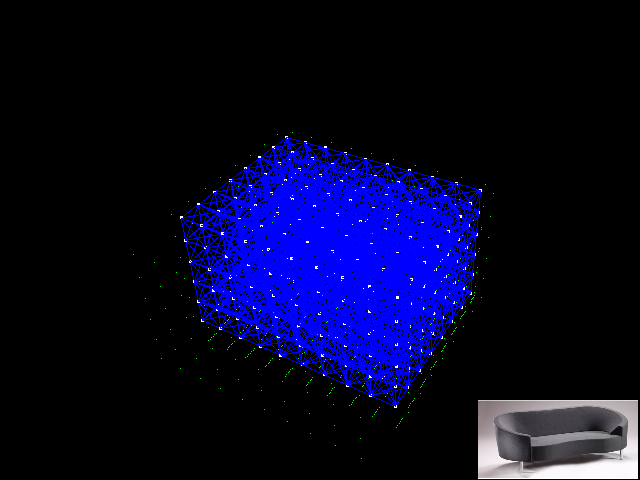
\includegraphics[width=0.33\linewidth]{fig/fluid1-00}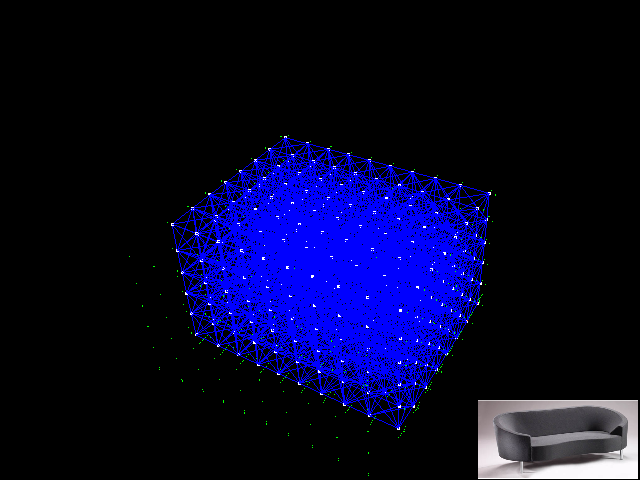
\includegraphics[width=0.33\linewidth]{fig/fluid1-01}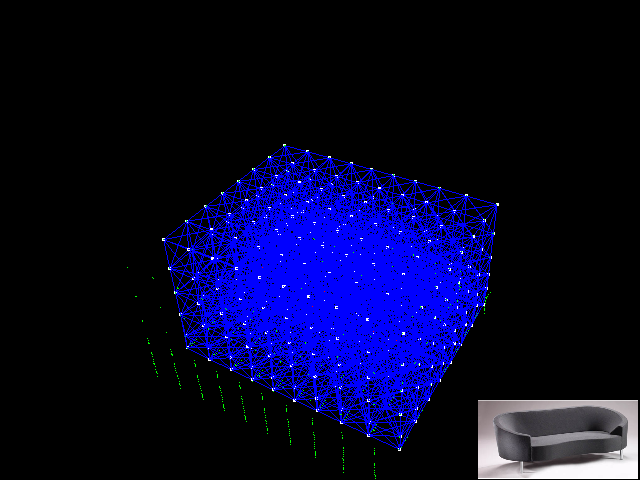
\includegraphics[width=0.33\linewidth]{fig/fluid1-02}\\
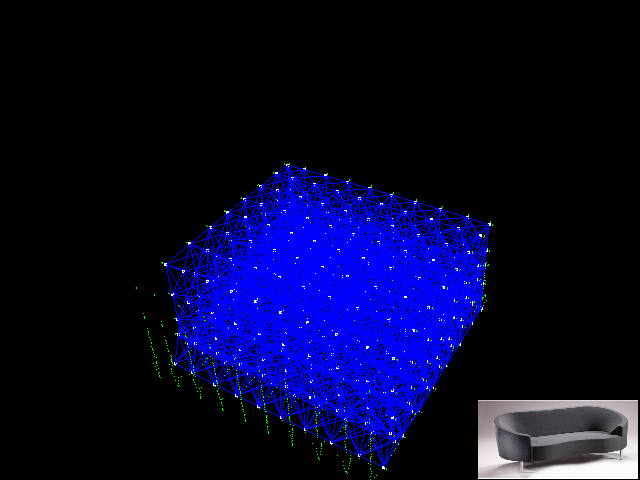
\includegraphics[width=0.33\linewidth]{fig/fluid1-03}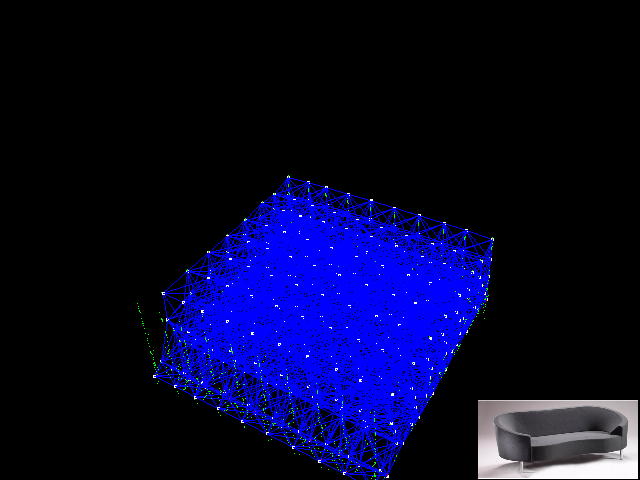
\includegraphics[width=0.33\linewidth]{fig/fluid1-04}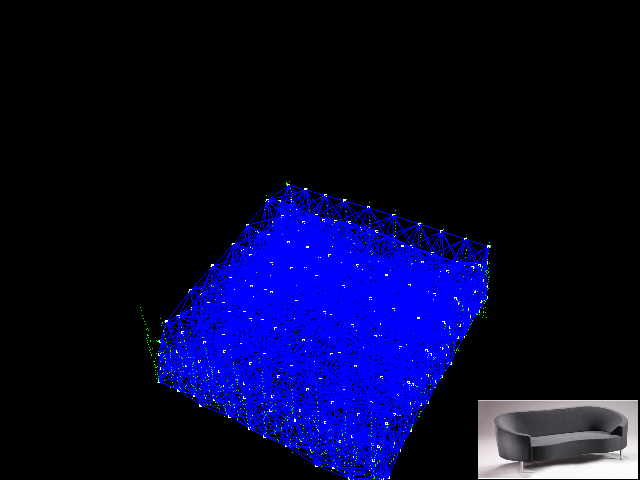
\includegraphics[width=0.33\linewidth]{fig/fluid1-05}\\
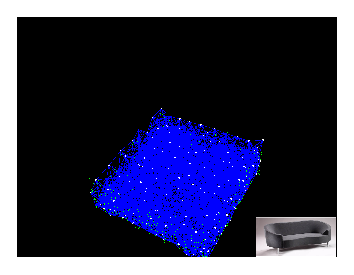
\includegraphics[width=0.33\linewidth]{fig/fluid1-06}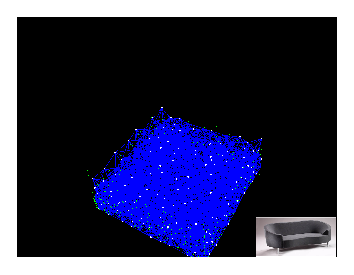
\includegraphics[width=0.33\linewidth]{fig/fluid1-07}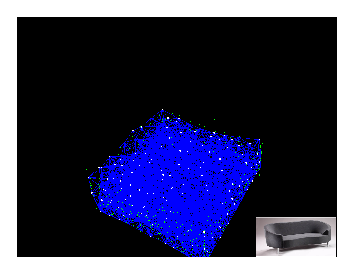
\includegraphics[width=0.33\linewidth]{fig/fluid1-08}\\
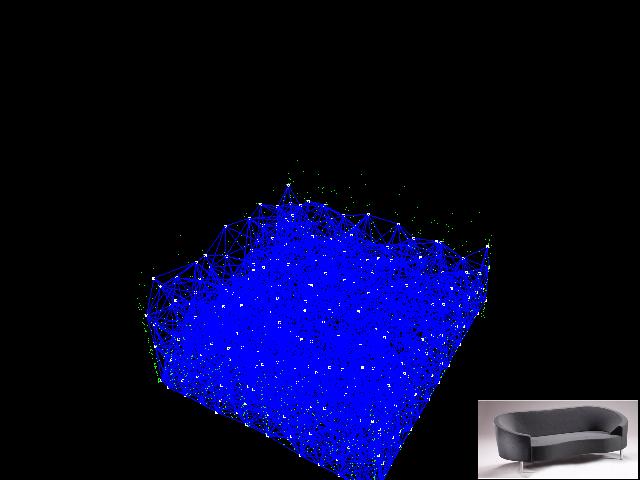
\includegraphics[width=0.33\linewidth]{fig/fluid1-09}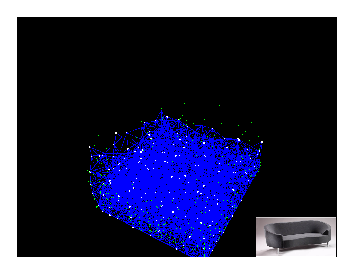
\includegraphics[width=0.33\linewidth]{fig/fluid1-10}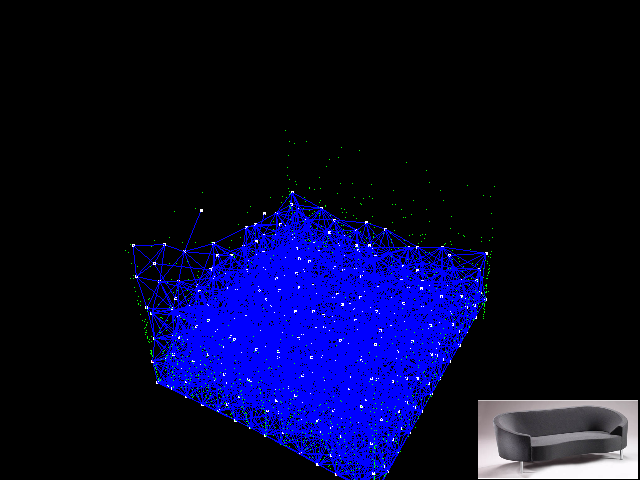
\includegraphics[width=0.33\linewidth]{fig/fluid1-11}
\caption{Fluid animation.}\label{fig:fluid1}
\end{figure}

The resulting animation is shown in figure~\ref{fig:fluid1}.

%
% \chapter{Physically-based animation} \label{chapter:pba}
\section{Particles} \label{sec:particles}
\subsection{Basic equation}
A particle is a moving point with a mass. Generally the mass is a constant over time while its position and velocity can vary. We therefore consider the mass $ m $ (in $ kg $) as an attribute while its position $ x $ (in $ m $) and its velocity $ v $ (in $m.s^{-1}$) are its state variables. 
Particles obey Newton's law: 
\begin{equation} \label{eq:newton}
ma = \Sigma f
\end{equation} 
where $a$ is the particle's acceleration (in $m.s^{-2}$). This defines the Ordinary Differential Equation (ODE) $a(t) = f(x,v,t)$. Physically-based animation requires us to repeatedly solve it over the interval $[t,t+dt]$ and redisplay.

From equation \ref{eq:newton} we can deduce $a=1/m\;\Sigma f$ and integrate time over a time step dt, and so on. The simplest integration method is Euler's explicit scheme:
\begin{eqnarray}
v(t+dt) &=& v(t)+a(t)dt \nonumber \\
x(t+dt) &=& x(t)+v(t)dt \label{eq:expliciteuler}
\end{eqnarray}

Particles can live in any k-dimensional space $\Re^k$, where state variables and forces are k-dimensional vectors of scalar values. The dynamics equation \ref{eq:newton} applies to each scalar value.
When considering $n$ particles the equations can be conveniently written in matrix form:
\begin{eqnarray*}
\ma M \ve a &=& \ve f\\
\ve a &=& \ma M^{-1} \ve f
\end{eqnarray*}
where \ma M is a diagonal matrix of dimension $kn\times kn$ , \ve a and \ve f are vectors of dimension $kn$ gathering all the scalar components associated with each particle.

Numerical integration can generate instabilities leading to the divergence of the simulated system. To avoid this, one solution is to decrease the time step. The other solution is to use an implicit integration scheme, which takes into account the variation of the forces during the time step. The simplest one is the implicit Euler's method which applies a step based on the forces at the end of the time step instead of the beginning. Equation \ref{eq:expliciteuler} becomes:
\begin{eqnarray}
v(t+dt) &=& v(t)+a(t+dt)dt \nonumber\\
x(t+dt) &=& x(t)+v(t+dt)dt \label{eq:impliciteuler}
\end{eqnarray}
Since $a(t+dt)$ is unknown we have to solve an equation.
If we write $v(t+dt) = v(t)+\Delta v$ the matrix form equation to solve is:
\begin{equation}
\label{eq:matimplicit}
\left( \ma M + dt \ma D + dt^2 \ma K \right) \ve{\Delta v} = dt \left( \ve f(t) + \ma D \ve{v}(t) \right) 
\end{equation}
where the damping matrix $\ma D = \delta \ve f/\delta \ve v$ encodes the variation of force given a variation of velocity, and the stiffness matrix $\ma K = \delta \ve f/\delta \ve p$ encodes the variation of force given a variation of position.

\subsection{Forces}
The forces are responsible for the accelerations of the bodies. Their physical unit is the Newton ($N=kg.m.s^{-2}$).
Here we briefly review the most commonly used forces.

\subsubsection{Weight}
A uniform gravitational field $g$ (in $m.s^{-2}$) applies a force 
\begin{equation} \label{eq:gravity}
f = mg
\end{equation} 
to each particle where $m$ is the mass of the particle.

\subsubsection{Linear damping}
Damping transforms kinetic energy to heat by applying a force opposed to the velocity. It tends to slow down the objects. Linear damping is proportional to the velocity, thus 
\begin{equation}\label{eq:lineardamping}
f=-\nu v
\end{equation}
where $v$ is the velocity of the particle and $\nu$ a positive scalar (in $kg.s^{-1}$).

\subsubsection{Air damping}
Air damping is proportional to the square of the velocity of the body with respect to the air:
\begin{equation}
f = -\rho S_u C_u v^2 u 
\end{equation}
where $\rho$ is the volumic mass the air ($kg.m^{-3}$), $v$ the velocity of the object, $u$ a no-dimensional unit vector in the direction of the velocity, $S$ the area ($m^2$) of the object projected along $u$, and $C_u$ a no-dimensional coefficient associated with the shape of the object and the direction $u$.

\subsubsection{Linear springs}
A springs applies an elastic force between two points. It is modeled using its rest length $l_0$ (in $m$) and its stiffness $k$ (in $N.m^{-1}$). 
Let $i$ and $j$ be the indices of points linked by a given spring. 
The force applied by a linear spring to point $i$ is given by:
\begin{equation}
\label{eq:spring}
f_i = k( l-l_0 ) u
\end{equation}
where $l=\|x_j - x_i\|$ is the distance between the points and $u$ a unit vector pointing from point $i$ to point $j$. The force $f_j$ applied to point $j$ is the opposite: $f_j = -f_i$. Nonlinear springs can be used to model more complex behaviors.

\subsubsection{Linear damped springs}
Damping forces are commonly associated with springs in order to dissipate energy. They are opposed to the relative velocity of the points. They are typically modeled using a coefficient $\nu$ (in $kg.s^{-1}$).
The force applied by a linear damped spring to point $i$ is given by:
\begin{equation}
\label{eq:dampedspring}
f_i = \left( k( l-l_0 ) + \nu v_{ij} \right) u
\end{equation}
where $v_{ij} = (v_j-v_i).u$ is the relative velocity of the particles along direction $u$.

\subsubsection{Finite elements}
Finite elements is a powerful paradigm for modeling continuous material. At our level, we can see them as springs acting on more than two points simultaneously. For example, a tetrahedral finite element acts on the four vertices of a tetrahedron and allows a more effective control of stiffness and volume than using springs.


%===========================================================================================

\section{Solids}
A solid is a moving reference frame with a mass matrix. In two dimensions it has three degrees of freedom (DOFs), two translations and one rotation, while in three dimensions it has six DOFs, three translations and three independent rotation values. The remainder of this document focuses on three dimensions.

\subsection{Orientation}
There are different ways of modeling orientation ot one frame with respect to another in three dimensions, each of them with advantages and drawbacks:
\begin{itemize}
\item matrices directly define the axes of the solid with respect to a reference frame. They allow fast projections from one frame to another but they contain nine dependent entries and they can not be set up intuitively;
\item Euler angles are compact (three parameters) and intuitive but they have singularities and they can not be easily combined;
 \item (axis, angle) pairs are more intuitive and more compact (four parameters) than matrices but they do not allow projections and combinations;
\item quaternions are compact (four parameters) and allow easy projections and combinations, but they are not easy to set up intuitively.
\end{itemize}

\subsubsection{Orientation matrices}
Orientations matrices are $3\times 3$ matrices, each column gathering the coordinates of one axis of the rotated frame with respect to the reference frame. Each column is thus a unit vector orthogonal to the others. This creates six relations among the nine parameters, leaving three independent DOFs.

\subsubsection{Euler angles}
Euler angles model a sequence of three rotations along three pairwise-independent directions. For example, the following matrix product represents a rotation $\alpha$ along axis $x$ followed by a rotation $\beta$ along rotated axis $y$ followed by a rotation $\gamma$ along the twice rotated axis $z$.
%\begin{equation}\label{eq:angles euler}
$$
\left(\begin{array}{ccc}
1 & 0 & 0 \\
0 & \cos\alpha & -\sin\alpha \\
0 & \sin\alpha &  \cos\alpha
\end{array}\right)
\left(\begin{array}{ccc}
\sin\beta & 0 &  \cos\beta\\
0 & 1 & 0 \\
\cos\beta & 0 & -\sin\beta
\end{array}\right)
\left(\begin{array}{ccc}
\cos\gamma & -\sin\gamma & 0\\
\sin\gamma & \cos\gamma & 0\\
0 & 0 & 1\\
\end{array}\right)
$$
%\end{equation}
Alternatively, this can be seen as a rotation  $\gamma$ along axis $z$ followed by a rotation $\beta$ along the fixed axis $y$ followed by a rotation $\alpha$ along the fixed axis $x$. An example of singularity is the fact that in this system, rotation $(\pi,\pi,0)$ is equivalent with rotation $(0,0,\pi)$. Another example is the fact that rotation $(\alpha,\pi /2, \gamma)$ is equivalent with rotation $(0,\pi /2, \alpha+\gamma)$ for any $\alpha$ and $\gamma$ (this loss of one DOF is called \emph{gimbal lock}).

\subsubsection{Axis, angle}
The rotation $\theta$ along an axis defined by a unit vector $n$ has the following matrix:
$$
\rot{\theta}{u} = \mat{I} + \sin\theta\oppvec{n} + (1-\cos\theta)\oppvec{n}^2
$$
where matrix $\oppvec{n}$  is the vector product matrix operator: 
%\begin{equation}\label{eq:oppvec}
$$
\oppvec{n} = \left(\begin{array}{ccc}
0 & -n_z & n_y \\
n_z & 0 & -n_x \\
-n_y & n_x & 0
\end{array}\right)
$$
%\end{equation}
It is possible to convert a matrix back to (axis, angle) by noticing that  $\trace{\mat R}=1+2\cos\theta$ et que $\mat R -\transp{\mat R} = 2\sin\theta\oppvec{n}$

\subsubsection{Quaternions}
Quaternions are an extension of complex numbers: $ \bm q = w + x\bm i + y \bm j + z \bm k = (w,\vect v)$.\\
w is the real part, \vect v the imagianry part.
Properties of \bm i, \bm j, \bm k:
$$
\begin{array}{l}
  \bm i^2 = \bm j^2 = \bm k^2 = -1\\
  \bm{ij}=\bm k,\;\bm{ji} = -\bm k\\
  \bm{jk}=\bm i,\;\bm{kj} = -\bm i\\
  \bm{ki}=\bm j,\;\bm{ik} = -\bm j\\
\end{array}
$$
A 3d vector is a pure imaginary quaternion:
$$
\bm p = (0,x,y,z)
$$
Product of quaternions (not commutative):
$$
\bm{q_1q_2} = (w_1w_2 - \bm v_1.\bm v_2, \; w_1\bm v_2 + w_2\bm v_1 + \bm v_1 \wedge \bm v_2)
$$
Conjugate quaternion:
$$
\begin{array}{l}
  \bm{\bar q} = w - x\bm i - y \bm j - z \bm k\\
  \bm{q\bar q} = w^2 + x^2 + y^2 + z^2
\end{array}
$$
Unit quaternions used to model rotations:
$$
\bm{q\bar q} = 1
$$
Rotation $(\theta, \bm u)$: {\em ($\bm u^2=1$)}
$$
\bm q_{(\theta,u)} = ( \cos{\frac{\theta}{2}}, u_x\sin{\frac{\theta}{2}}, u_y\sin{\frac{\theta}{2}}, u_z\sin{\frac{\theta}{2}})
$$
Rotation of a vector \bm p:$\;\;\;\bm{ qp\bar{q} }$\\
Rotation matrix associated with a unit quaternion:
$$
\left( \begin{array}{ccc}
  1 - 2y^2 - 2z^2 & 2xy - 2wz & 2xz + 2wy \\
  2xy + 2wz & 1-2x^2-2z^2 & 2yz - 2wx \\
  2xz - 2wy & 2yz + 2wx & 1 - 2x^2 - 2y^2
\end{array} \right)
$$
Combination of rotations: $\rot{\alpha}{u}\rot{\beta}{v} \longrightarrow q_{(\alpha,u)}q_{(\beta,v)}$\\
Inverse rotation: $\inv{ q_{(\theta,u)}} = q_{(-\theta,u)} = q_{(\theta,-u)} = (-w,\vect v) = (w,\vect -v)$ \\
Conversion $(w, \vect v) \longrightarrow ( \theta, \vect u)$ :
\begin{eqnarray*}
\cos(\theta/2) &=& w\\
\sin(\theta/2) &=& \|\vect v\|\\
\vect u &=& \vect v/\|\vect v\|
\end{eqnarray*}

The time derivative of the unit quaternion $q$ defining the orientation of a solid with angular velocity $\omega$ (vector of $\RRR$, see section \ref{sec:omega}) is: $\dot q = \frac{1}{2}\omega q$.


\subsection{Kinematics}
\todo{choose omega or Omega. Simplify notations where possible.}
\todo{choose n or u.}
\subsubsection{Derivative in \Rep{0} of a vector fixed in \Rep{1}. Angular velocity.} \label{sec:omega}
Consider vector \fixedans{\vect u}{1}, fixed in frame \rep{1}. Frame \rep{1} rotates with respect to frame \rep{0}. Consider the projection \vecin{\fixedans{\vect u}{1}}{0} of this vector to \rep{0}, which we sometimes call \vect u for clarity, and its derivative in \rep{0} which we write $\derivedans{\fixedans{\bm u}{1}}{0}$.


Let \mat{R(dt)} be the rotation of \rep{1} between time $t$ and $t+dt$. We write:
\begin{eqnarray}
 \vect u(t+dt) &=& \mat{R(dt)} \vect u(t)\\
 \vect u(t+dt) - \vect u(t)&=& (\mat{R(dt)}-\ident{}) \vect u(t) \label{eq ri}
\end{eqnarray}
Let $\dot{\theta}$ be the angular velocity along the rotation axis, which we set to \vect z for clarity. The first-order Taylor series is: 
$$
 \mat{R(dt)}-\ident{} = 
 \left(\begin{array}{ccc}
  cos(\dot{\theta}dt)-1 & -sin(\dot{\theta}dt) & 0\\   
   sin(\dot{\theta}dt)& cos(\dot{\theta}dt)-1& 0\\ 
  0 & 0 & 0 
 \end{array}\right)
 \longrightarrow
 \left(\begin{array}{ccc}
  0 & -\dot{\theta}dt & 0\\
  \dot{\theta}dt & 0 & 0\\
  0 & 0 & 0
 \end{array}\right) 
 =
 \dot{\theta}dt \oppvec{z}
$$
which can be easily extended to any rotation axis. Let $\vecrot{1}{0}=\dot{\theta}\vect n$. Dividing expression \ref{eq ri} by $dt$ and decreasing $dt$ to $0$ gives $\dot{\mat R} = \oppvec{ \vecrot{1}{0} }$.

We can write the time derivative in \rep{0}: $\derivedans{\fixedans{\bm u}{1}}{0}  = \vecrot{1}{0} \wedge  \fixedans{\vect u}{1}$, or more simply:

\begin{equation}\label{vrot}
\begin{array}{rcl}
 \dot{\vect u} &=& \dot{\mat R} \vect u \\
               &=& \oppvec{ \vecrot{1}{0} } \vect u \\
               &=& \vecrot{1}{0} \wedge \vect u
\end{array}
\end{equation}
 

\subsection{Velocity in \Rep{0} of a point fixed in \Rep{1}. Velocity field.}
We consider the velocity $\vfdans{A}{1}{0}$ in \rep{0} of a point $A$ fixed in \rep{1} while \rep{1} moves with respect to \rep{0}. Let $O_0$ be the origin of \rep{0} and $O_1$ the origin of \rep{1}. The following relation holds:
$$ \vfdans{A}{1}{0} = \vfdans{O_1}{1}{0} + \vecrot{1}{0} \wedge \vecf{O_1A} \label{eq vit} \label{eq vit solide}
$$

\subsection{Acceleration in \Rep{0} of  point fixed in \Rep{1}. Acceleration field. }
By deriving equation \ref{eq vit}, and based on the fact that $\vecf{O_1A}$ is fixed in \rep{1}, we get the acceleration of A, fixed in \rep{1}, with respect to \rep{0}:
\begin{equation}\label{eq acc}
 \afdans{A}{1}{0} = \afdans{O_1}{1}{0} + \accrot{1}{0}\wedge \vecf{O_1A} + \vecrot{1}{0} \wedge \left( \vecrot{1}{0} \wedge \vecf{O_1A} \right)
\end{equation}

\subsection{Derivative in \rep{0} of a vector defined in \rep{1}}
Let $(\vect e_1, \vect e_e, \vect e_3)$ be a base of \rep{1}. We have:
\begin{eqnarray*}
 \vecin{u}{1} &=& \sum_i x_i \vect e_i\\
 \dot{\vect u} &=& \sum_i \dot x_i \vect e_i + \sum_i x_i \dot{\vect e}_i
\end{eqnarray*}
and thus:
\begin{equation}\label{eq vec mob}
 \derivedans{u}{0} = \derivedans{u}{1} + \vecrot{1}{0} \wedge \vect u
\end{equation}


\subsection{Velocity in \rep{0} of a point moving in \rep{1}.}
Let \vmdans{A}{1} be the velocity of point $A$ with respect to \rep{1}. We have:
\begin{equation}\label{eq vit mob}
\vmdans{A}{0} = \vmdans{A}{1} + \vfdans{O_1}{1}{0} + \vecrot{1}{0} \wedge \vecf{O_1A}
\end{equation}
Note that $O_1$ being the origin of frame \rep{1}, we have $\vmdans{O_1}{0} = \vfdans{O_1}{1}{0}$.

\subsection{Acceleration in \rep{0} of a point moving in \rep{1}. Coriolis acceleration.}
EBy deriving equation \ref{eq vit mob} nous we get:
$$
 \amdans{A}{0} = \underbrace{\amdans{A}{1} + \vecrot{1}{0}\wedge \vmdans{A}{1}}_{\overset{\circ}{\vmdans{A}{1}}} + \amdans{O_1}{0} + \underbrace{\accrot{1}{0}\wedge \vect{O_1}{A} + \vecrot{1}{0}\wedge \vmdans{A}{1} + \vecrot{1}{0} \wedge (\vecrot{1}{0}\wedge \vecf{O_1A})}_{\overset{\circ}{\vecrot{1}{0} \wedge \vecf{O_1A}}}
$$
or:
\begin{equation}\label{eq acc mob}
 \amdans{A}{0} = \amdans{A}{1} +  \amdans{O_1}{0} + \vecrot{1}{0} \wedge (\vecrot{1}{0}\wedge \vecf{O_1A}) + 2\vecrot{1}{0}\wedge \vmdans{A}{1}
\end{equation}
with:
\begin{itemize}
\item $\amdans{A}{1} = \sum_i \ddot x_i \vect e_i$ relative acceleration
\item $\amdans{O_1}{0}$ frame acceleration (?)
\item $\vecrot{1}{0} \wedge (\vecrot{1}{0}\wedge \vecf{O_1A})$ centripetal acceleration
\item $2\vecrot{1}{0}\wedge \vmdans{A}{1}$ Coriolis acceleration
\end{itemize}


\subsection{Dynamics}
Solids accelerate linearly due to forces, and accelerate angularly due to torques. A given torque has the same value everywhere in the solid. However, a given force generates different torques at different points. The torque $\tau$ applied at point $c$ generated by a force $f$ applied at point $b$ is: $\tau=cb\wedge f$.

The acceleration $\ddot c$ of the mass center of a solid and its angular acceleration $\dot \omega$ with respect to the world are given by the relations:

    \begin{eqnarray*}
        m \bf{ \ddot c } = \sum\bf{f_{ext}} \\%\label{eq:PFD1}\\
        \bf{ I_M \dot \omega } + \bm{ \omega \times I_M \omega} = \sum\bf{\tau_{ext}} %\label{eq:PFD2}
    \end{eqnarray*}
where $m$ is the mass of the solid, $\sum {\bf f_{ext}}$ is the sum of the forces applied to the solid, ${\bf I_M}$ is the inertia matrix et $\sum {\bf \tau_{ext}}$ the sum of the torques applied to the solid and expressed at its mass center. The inertia matrix is given by:
$${\bf I_M} = \int_x \int_y \int_z \rho (x,y,z)\begin{bmatrix}  y^2+z^2 & -xy & -xz \\ -xy & x^2+z^2 & -yz \\ -xz & -yz & x^2+y^2 \end{bmatrix} dx dy dz$$
where $\rho(x,y,z)$ is the volumic mass of the naterial (in $kg.m^{-3}$).



%
% \appendix
\chapter{Appendices} \label{chap:appendices}

\section{Mechanical class diagrams} \label{sec:umlmeca}
Figure \ref{fig:umlMechClasses} shows the mechanical classes of \sofa. Not all members and methods are shown. For a full list, please refer to the source code documentation.

\begin{figure}[htp]
	\hspace{-2cm}
	\includegraphics*[width=20cm]{fig/uml-mechanical-classes.eps}  
\label{fig:umlMechClasses} 
\caption{Class diagram of the mechanics.}
\end{figure}

	%\setlength{\textwidth }{16cm}	% largeur de ligne

